\documentclass[oneside]{book}

\usepackage[utf8]{inputenc}
\usepackage[T2A]{fontenc}
\usepackage[russian]{babel}
\usepackage[left = 0.3\textwidth, right = 0.3\textwidth]{geometry}
\usepackage{parskip}
\usepackage[fleqn]{amsmath}
\usepackage{mathtools}
\usepackage{amsfonts}
\usepackage{amssymb}
\usepackage{graphicx}
\usepackage{hyperref}
\usepackage{bookmark}
\usepackage{textcomp}

\setlength{\parskip}{0.03\textheight}

\graphicspath{{images/}}

\hypersetup{
    colorlinks,
    citecolor=black,
    filecolor=black,
    linkcolor=black,
    urlcolor=black
}

\newcommand{\meta}[1]{\text{<}#1\text{>}}
\newcommand{\sequence}[1]{\left\{#1\right\}}
\newcommand{\set}[1]{\left\{#1\right\}}
\newcommand{\simsub}{\stackrel{<}{\thicksim}}

\title{Математика}
\date{\today}
\author{Мы}

\begin{document}
	\maketitle
    \tableofcontents
	\chapter{Примечания}
    В данном материале очень много опечаток.
    А также данный материал неконсистентен -
    он не стандартизирован.

	Чтобы понять, что означают '<', '>',
	попробуйте их убрать.

	\chapter{Логика}
	\begin{flalign*}
		\forall A, \ B \
		\left(
		A \longrightarrow B
		\Leftrightarrow
		\left\{
		\begin{aligned}
			&\text{Из посылки} \ A \ \text{вытекает вывод} \ B. \\
			&A - \text{достаточное условие для} \ B. \\
			&B - \text{необходимое условие для} \ A. \\
		\end{aligned}
		\right.
		\right)
	\end{flalign*}

	\begin{flalign*}
		\forall A, \ B \
		\left(
		\left\{
		\begin{aligned}
			&A \longrightarrow B \\
			&B \longrightarrow A
		\end{aligned}
		\right.
		\Leftrightarrow
		A \ \text{и} \ B - \text{логически эквивалентные утверждения.}
		\right)
	\end{flalign*}

	\begin{flalign*}
		\forall A, \ B \
		(
		(A \longrightarrow B) \ - \ \text{прямое утверждение}.
		\Leftrightarrow
		(B \longrightarrow A) \ - \ \text{обратное утверждение}.
		)
	\end{flalign*}

	\begin{flalign*}
		\forall A, \ B \
		(
		(A \longrightarrow B) \ - \ \text{прямое утверждение}.
		\Leftrightarrow
		(\overline{A} \longrightarrow \overline{B}) \ - \ \text{противоположное утверждение}.
		)
	\end{flalign*}

	\begin{flalign*}
		\forall A, \ B \
		(
		(A \longrightarrow B) \ - \ \text{прямое утверждение}.
		\Leftrightarrow
		(\overline{B} \longrightarrow \overline{A}) \ - \ \text{противоположное обратному утверждение}.
		)
	\end{flalign*}

	\begin{flalign*}
		\forall A, \ B \
		\left(
		\left\{
		\begin{aligned}
			&A - \text{прямое утверждение.} \\
			&B - \text{противоположное обратному утверждение.}
		\end{aligned}
		\right.
		\longrightarrow
		A \Leftrightarrow B
		\right)
	\end{flalign*}

	\textbf{Доказательство от противного:}
	\begin{flalign*}
		\forall A \ \exists B \ (
		B \wedge (\overline{A} \longrightarrow \overline{B})
		\longrightarrow
		A
		)
	\end{flalign*}

	\textbf{Принцип математической индукции (ПМИ):}
	\begin{flalign*}
		\forall f \
		\left(
		\forall n \
		\left\{
		\begin{aligned}
			&f: \mathbb{N} \longrightarrow Bool \\
			&f(0) \\
			&f(n) \longrightarrow f(n + 1)
		\end{aligned}
		\right.
		\longrightarrow
		\forall n \
		f(n)
		\right)
	\end{flalign*}

	\begin{flalign*}
		\forall f \
		Prog(f) - \text{прогрессивность свойства} \ f.
	\end{flalign*}

	\begin{flalign*}
		\forall f, \ g \
		\left(
		\left\{
		\begin{aligned}
			&f: \mathbb{N} \longrightarrow Bool \\
			&g: \mathbb{N} \longrightarrow Bool \\
			&f(g) = \forall n \ \left(\forall m \ \left(m < n \longrightarrow g(m)\right) \longrightarrow g(n)\right)
		\end{aligned}
		\right.
		\Leftrightarrow
		f = Prog(g)
		\right)
	\end{flalign*}

	\textbf{Принцип сильной индукции (ПСИ):}
	\begin{flalign*}
		\forall f \
		\left(
		Prog(f)
		\longrightarrow
		\forall n \ f(n)
		\right)
	\end{flalign*}

	\textbf{Принцип наименьшего числа (ПНЧ):}
	\begin{flalign*}
		\forall f \
		\left(
		\exists m \
		\left\{
		\begin{aligned}
			&f: \mathbb{N} \longrightarrow Bool \\
			&f(m)
		\end{aligned}
		\right.
		\longrightarrow
		\exists n \ \forall a \
		\left\{
		\begin{aligned}
			&f(n) \\
			&a < n \longrightarrow \overline{f(a)}
		\end{aligned}
		\right.
		\right)
	\end{flalign*}

	\chapter{Множества}
	\section{Аксиомы множеств}
	\begin{flalign*}
		\forall a \
		a - \text{множество}.
	\end{flalign*}

	\begin{flalign*}
		\forall a, \ b \
		\left[
		\begin{aligned}
			&b \in a \\
			&b \notin a
		\end{aligned}
		\right.
	\end{flalign*}

	\textbf{Аксиома основания:} \\
	Не бывает бесконечных цепочек вида
	\begin{math}
		\left\{
		\begin{aligned}
			&x_1 \in x_2 \\
			&x_2 \in x_3 \\
			&\vdots
		\end{aligned}
		\right.
	\end{math}

	\textbf{Аксиома равенства:}
	\begin{flalign*}
		\forall a, \ b \
		\left(
		a = b
		\Leftrightarrow
		\forall c \
		\left(
		a \in c \Leftrightarrow b \in c
		\right)
		\right)
	\end{flalign*}

	\begin{flalign*}
		\forall a_1, \ a_2, \ \ldots, \ a_n \
		\exists a \
		a = \set{a_1, a_2, \ldots, a_n}
	\end{flalign*}

	\begin{flalign*}
		\forall a_1, \ a_2, \ \ldots, \ a_n \ b \
		\left(
		b \in \set{a_1, a_2, \ldots, a_n}
		\Leftrightarrow
		\left[
		\begin{aligned}
			&b = a_1 \\
			&b = a_2 \\
			&\vdots \\
			&b = a_n
		\end{aligned}
		\right.
		\right)
	\end{flalign*}

	\begin{flalign*}
		\forall f, \ c \
		\left(
		f: c \longrightarrow Bool
		\Leftrightarrow
		\exists b \
		b = \set{a \in c \mid f(a)}
		\right)
	\end{flalign*}

	\begin{flalign*}
		\forall f, \ b, \ c \
		\left(
		c \in \set{a \in b \mid f(a)}
		\Leftrightarrow
		\left\{
		\begin{aligned}
			&c \in b \\
			&f(c)
		\end{aligned}
		\right.
		\right)
	\end{flalign*}

	\section{Другое}
	\begin{flalign*}
		\forall a, \ b \
		\left(
		a \subseteq b
		\Leftrightarrow
		\forall c \
		\left(
		c \in a \longrightarrow c \in b
		\right)
		\right)
	\end{flalign*}

    \begin{flalign*}
        \forall a, \ c \
        \left(
        a \subset c
        \Leftrightarrow
        c - \text{собственное подмножество} \ a.
        \right)
	\end{flalign*}

	\begin{flalign*}
		\forall a, \ b \
		\left(
		a = b
		\Leftrightarrow
		\forall c \
		\left(
		c \in a \Leftrightarrow c \in b
		\right)
		\right)
	\end{flalign*}

	\begin{flalign*}
		\forall a, \ b \
		\left(
		a = b
		\Leftrightarrow
		\forall f \
		\left(
		\exists c \
		f: c \longrightarrow Bool
		\longrightarrow
		\left(
		f(a) \Leftrightarrow f(b)
		\right)
		\right)
		\right)
	\end{flalign*}

	\begin{flalign*}
		\forall a, \ b \
		\left(
		a = b
		\Leftrightarrow
		\left\{
		\begin{aligned}
			&a \subseteq b \\
			&b \subseteq a
		\end{aligned}
		\right.
		\right)
	\end{flalign*}

	\begin{flalign*}
		a \subseteq a
	\end{flalign*}

	\begin{flalign*}
		\forall a, \ c \
		\left(
		\exists b \
		\left\{
		\begin{aligned}
			&a \subseteq b \\
			&b \subseteq c
		\end{aligned}
		\right.
		\longrightarrow
		a \subseteq c
		\right)
	\end{flalign*}

	\begin{flalign*}
		\forall a \
		a \notin \varnothing
	\end{flalign*}

	\begin{flalign*}
		\forall a \
		\varnothing \subseteq a
	\end{flalign*}

	\textbf{Парадокс Рассела:}
	\begin{flalign*}
		\overline{\exists a \ \forall b \ \left(b \in a \Leftrightarrow b \notin b\right)}
	\end{flalign*}

	\begin{flalign*}
		\forall a, \ b \
		\left(
		a \in P(b)
		\Leftrightarrow
		a \subseteq b
		\right)
	\end{flalign*}

	\begin{flalign*}
		\forall a, \ b, \ c \
		\left(
		c \in a \cup b
		\Leftrightarrow
		\left[
		\begin{aligned}
			&c \in a \\
			&c \in b
		\end{aligned}
		\right.
		\right)
	\end{flalign*}

	\begin{flalign*}
		\forall a, \ c \
		\left(
		a \in \cup b
		\Leftrightarrow
		\exists c \
		\left\{
		\begin{aligned}
			&a \in c \\
			&c \in b
		\end{aligned}
		\right.
		\right)
	\end{flalign*}

	\begin{flalign*}
		\forall a, \ b \
		a \cap b = \set{c \in a \mid c \in b}
	\end{flalign*}

	\begin{flalign*}
		\forall a, \ b \
		a \diagdown b = \set{c \in a \mid c \notin b}
	\end{flalign*}

	\begin{flalign*}
		\forall a, \ b \
		a \subseteq b \Leftrightarrow a \cap b = a
	\end{flalign*}

	\begin{flalign*}
		\forall a, \ b \
		a \subseteq b \Leftrightarrow a \cup b = b
	\end{flalign*}

	\begin{flalign*}
		\forall a, \ b \
		\left(
		b - \text{universum}.
		\Leftrightarrow
		\overline{a} = b \diagdown a
		\right)
	\end{flalign*}

	\begin{flalign*}
		\cup - \text{операция, обладающая коммутативным свойством}.
	\end{flalign*}

	\begin{flalign*}
		\cup - \text{операция, обладающая ассоциативным свойством}.
	\end{flalign*}

	\begin{flalign*}
		\cup - \text{операция, обладающая дистрибутивным свойством с} \ \cap.
	\end{flalign*}

	\begin{flalign*}
		\cap - \text{операция, обладающая коммутативным свойством}.
	\end{flalign*}

	\begin{flalign*}
		\cap - \text{операция, обладающая ассоциативным свойством}.
	\end{flalign*}

	\begin{flalign*}
		\cap - \text{операция, обладающая дистрибутивным свойством с} \ \cup.
	\end{flalign*}

	\begin{flalign*}
		\forall a, \ b \
		(a, b) = \set{\set{a}, \set{a, b}}
	\end{flalign*}

	\begin{flalign*}
		\forall a, \ b, \ c \
		\left(
		\left\{
		\begin{aligned}
			&a \in c \\
			&b \in c
		\end{aligned}
		\right.
		\longrightarrow
		(a, b) \in P\left(P\left(c\right)\right)
		\right)
	\end{flalign*}

	\begin{flalign*}
		a \times b
		=
		\set
		{
			z \in P(P(a \cup b))
			\mid
			\exists x, \ y \
			\left\{
			\begin{aligned}
				&x \in a \\
				&y \in b \\
				&z = (x, y)
			\end{aligned}
			\right.
		}
	\end{flalign*}

	\begin{flalign*}
		a^0 = \set{\varnothing}
	\end{flalign*}

	\begin{flalign*}
		\forall a_1, \ a_2, \ \ldots, \ a_n \
		\left(a_1, a_2, a_3, \ldots, a_n\right)
		=
		\left(\left(\left(a_1, a_2\right), a_3\right) \ldots a_n \right)
	\end{flalign*}
    
    \chapter{Бинарные отношения}
    \begin{flalign*}
        \forall A, \ B, \ C \
        \left(
        C \subseteq A \times B
        \Leftrightarrow
        C - \text{множество бинарных отношений между множествами} \ A \ \text{и} \ B.
        \right)
	\end{flalign*}
    \begin{flalign*}
        \forall A, \ B, \ C \
        \left(
        C \subseteq A \times B
        \Leftrightarrow
        dom \ C = \set{x \in A \mid \exists y \ (x, y) \in C}
        \right)
	\end{flalign*}
    \begin{flalign*}
        \forall A, \ B, \ C \
        \left(
        C \subseteq A \times B
        \Leftrightarrow
        rng \ C = \set{y \in B \mid \exists x \ (x, y) \in C}
        \right)
	\end{flalign*}
    \begin{flalign*}
        \forall A, \ B, \ C \
        \left(
        C \subseteq A \times B
        \Leftrightarrow
        C^{-1} = \set{(y, x) \in B \times A \mid (x, y) \in C}
        \right)
	\end{flalign*}
    \begin{flalign*}
        \forall A, \ B, \ C \
        \left(
        C \subseteq A \times B
        \Leftrightarrow
        \forall x, \ y \
        \left(
        x C y
        \Leftrightarrow
        (x, y) \in C
        \right)
        \right)
	\end{flalign*}
    \begin{flalign*}
        \forall A, \ B, \ C, \ Q, \ Z \
        \left(
        \left\{
        \begin{aligned}
            &C \subseteq A \times Z \\
            &Q \subseteq Z \times B
        \end{aligned}
        \right.
        \Leftrightarrow
        Q \circ C = \set
        {
        (x, y) \in dom \ C \times rng \ Q
        \mid
        \exists z \
        \left\{
        \begin{aligned}
            &x C z \\
            &z Q y
        \end{aligned}
        \right.
        }
        \right)
	\end{flalign*}
    \begin{flalign*}
        \forall A, \ B, \ C, \ Q, \ Z \
        \left(
        \left\{
        \begin{aligned}
            &C \subseteq A \times Z \\
            &Q \subseteq Z \times B
        \end{aligned}
        \right.
        \Leftrightarrow
        \left( Q \circ C \right)^{-1} = C^{-1} \circ Q^{-1}
        \right)
    \end{flalign*}
    \begin{flalign*}
        \forall A \
        id_{A} = \set{z \in A \times A \mid \exists x \ z = (x, x)}
    \end{flalign*}
    \begin{flalign*}
        \forall A, \ B, \ C \
        \left(
        C \subseteq A \times B
        \longrightarrow
        \left\{
        \begin{aligned}
            &id_{B} \circ C = C \\
            &C \circ id_{A} = C
        \end{aligned}
        \right.
        \right)
	\end{flalign*}
    \begin{flalign*}
        \forall A, \ B, \ C \
        \left(
        C \subseteq A \times B
        \longrightarrow
        \left\{
        \begin{aligned}
            &id_{B} \circ C = C \\
            &C \circ id_{A} = C
        \end{aligned}
        \right.
        \right)
	\end{flalign*}
    \begin{flalign*}
        \forall C, \ X \
        \left(
        \exists A, \ B \
        C \subseteq A \times B
        \Leftrightarrow
        C[X] - \text{образ множества $ X $ под действием отношения $ C $}.
        \right)
	\end{flalign*}
    \begin{flalign*}
        \forall C, \ X \
        C[X] = \set
        {
        b \in rng \ C
        \mid
        \exists a \
        \left\{
        \begin{aligned}
            &a \in X \\
            &a C b
        \end{aligned}
        \right.
        }
	\end{flalign*}
    \begin{flalign*}
        \forall C \
        C[dom \ C] = rng \ C
	\end{flalign*}
    \begin{flalign*}
        \forall C, \ X \
        \left(
        C[X] - \text{образ множества $ X $ под действием отношения $ C $}.
        \Leftrightarrow
        C^{-1}[X] - \text{пробраз множества $ X $ под действием отношения $ C $}.
        \right)
	\end{flalign*}
    \begin{flalign*}
        \forall C \
        C^{-1}[rng \ C] = dom \ C
	\end{flalign*}
    \begin{flalign*}
        \forall C \
        C[\varnothing] = \varnothing
	\end{flalign*}
    \begin{flalign*}
        \forall C, \ X, \ Y \
        C[X \cup Y] = C[X] \cup C[Y]
	\end{flalign*}
    \begin{flalign*}
        \forall C, \ X, \ Y \
        C[X \cap Y] \subseteq C[X] \cap C[Y]
	\end{flalign*}
    \begin{flalign*}
        \forall C, \ X, \ Y \
        \left( Q \circ C \right)[X] = Q[C[X]]
	\end{flalign*}
    \begin{flalign*}
        \forall R \
        \left(
        \forall x, \ y, \ z \
        \left(
        \left\{
        \begin{aligned}
            &x R y \\
            &x R z
        \end{aligned}
        \right.
        \longrightarrow
        y = z
        \right)
        \Leftrightarrow
        R - \text{функционально}.
        \right)
	\end{flalign*}
    \begin{flalign*}
        \forall R \
        \left(
        \forall x, \ y, \ z \
        \left(
        \left\{
        \begin{aligned}
            &y R x \\
            &z R x
        \end{aligned}
        \right.
        \longrightarrow
        y = z
        \right)
        \Leftrightarrow
        R - \text{инъективно}.
        \right)
	\end{flalign*}
    \begin{flalign*}
        \forall R \
        \left(
        \forall x, \ y, \ z \
        \left(
        R - \text{функционально}.
        \Leftrightarrow
        R^{-1} - \text{инъективно}.
        \right)
        \right)
	\end{flalign*}
    \begin{flalign*}
        \forall R, \ X \
        \left(
        X \subseteq dom \ R
        \Leftrightarrow
        R - \text{тотально для} \ X.
        \right)
	\end{flalign*}
    \begin{flalign*}
        \forall R, \ Y \
        \left(
        Y \subseteq rng \ R
        \Leftrightarrow
        R - \text{сюрьективно для} \ Y.
        \right)
	\end{flalign*}
    \begin{flalign*}
        \forall R, \ X \
        \left(
        R - \text{тотально для} \ X.
        \Leftrightarrow
        R^{-1} - \text{сюрьективно для} \ X.
        \right)
	\end{flalign*}
    \begin{flalign*}
        \forall R, \ Q \
        \left(
        \left\{
        \begin{aligned}
            &R - \text{функционально}. \\
            &Q - \text{функционально}.
        \end{aligned}
        \right.
        \longrightarrow
        R \circ Q - \text{функционально}.
        \right)
	\end{flalign*}
    \begin{flalign*}
        \forall R, \ Q \
        \left(
        \left\{
        \begin{aligned}
            &R - \text{инъективно}. \\
            &Q - \text{инъективно}.
        \end{aligned}
        \right.
        \longrightarrow
        R \circ Q - \text{инъективно}.
        \right)
	\end{flalign*}
    \begin{flalign*}
        \forall R, \ Q, \ A \
        \left(
        \exists B \
        \left\{
        \begin{aligned}
            &Q \subseteq A \times B \\
            &R - \text{тотально для} \ rng \ Q. \\
            &Q - \text{тотально для} \ A.
        \end{aligned}
        \right.
        \longrightarrow
        R \circ Q - \text{тотально для} \ A.
        \right)
	\end{flalign*}
    \begin{flalign*}
        \forall R, \ Q, \ C \
        \left(
        \exists B \
        \left\{
        \begin{aligned}
            &R \subseteq B \times C \\
            &Q - \text{сюрьективно для} \ dom \ R. \\
            &R - \text{сюрьективно для} \ C.
        \end{aligned}
        \right.
        \longrightarrow
        R \circ Q - \text{сюрьективно для} \ C.
        \right)
	\end{flalign*}
    \begin{flalign*}
        \forall A, \ R \
        \left(
        \exists B
        \left\{
        \begin{aligned}
            &R: A \longrightarrow B \\
            &R - \text{инъекция}.
        \end{aligned}
        \right.
        \Leftrightarrow
        R^{-1} \circ R \subseteq id_A
        \right)
	\end{flalign*}
    \begin{flalign*}
        \forall B, \ R \
        \left(
        \exists A
        \left\{
        \begin{aligned}
            &R: A \longrightarrow B \\
            &R - \text{функционально}.
        \end{aligned}
        \right.
        \Leftrightarrow
        R \circ R^{-1} \subseteq id_B
        \right)
	\end{flalign*}
    \begin{flalign*}
        \forall A, \ R \
        \left(
        \exists B
        \left\{
        \begin{aligned}
            &R: A \longrightarrow B \\
            &R - \text{тотально для} \ A.
        \end{aligned}
        \right.
        \Leftrightarrow
        id_A \subseteq R^{-1} \circ R
        \right)
	\end{flalign*}
    \begin{flalign*}
        \forall B, \ R \
        \left(
        \exists A
        \left\{
        \begin{aligned}
            &R: A \longrightarrow B \\
            &R - \text{сюрьективна для} \ B.
        \end{aligned}
        \right.
        \Leftrightarrow
        id_B \subseteq R \circ R^{-1}
        \right)
	\end{flalign*}
    
	\chapter{Общая алгебра}
	\begin{flalign*}
		\forall A, \ * \
		\left(
		\left\{
		\begin{aligned}
			&* - \text{операция}. \\
			&*: A \times A \longrightarrow A
		\end{aligned}
		\right.
		\Leftrightarrow
		* - \text{бинарная операция на множестве} \ A.
		\right)
	\end{flalign*}
	\begin{flalign*}
		\forall A, \ * \
		\left(
		\left(A, *\right)
		\Leftrightarrow
		* - \text{бинарная операция на множестве} \ A.
		\right)
	\end{flalign*}
	\begin{flalign*}
		\forall A, \ * \
		\left(
		\left(A, *\right)
		\Leftrightarrow
		A - \text{группоид (магма)}.
		\right)
	\end{flalign*}
	\begin{flalign*}
		\forall A, \ * \
		\left(
		\forall a, \ b, \ c \
		\left\{
		\begin{aligned}
			&(*, A) \\
			&a, b \in A \longrightarrow a * b = b * a
		\end{aligned}
		\right.
		\Leftrightarrow
		* - \text{бинарная ассоциативная операция на множестве} \ A.
		\right)
	\end{flalign*}
	\begin{flalign*}
		\forall A, \ * \
		\left(
		\forall a, \ b, \ c \
		\left\{
		\begin{aligned}
			&(*, A) \\
			&a, b, c \in A \longrightarrow (a * b) * c = a * (b * c)
		\end{aligned}
		\right.
		\Leftrightarrow
		\begin{aligned}
			&* - \text{бинарная коммутативная операция на} \\
			&\text{множестве} \ A.
		\end{aligned}
		\right)
	\end{flalign*}
	\begin{flalign*}
		\forall A, \ * \
		\left(
		\begin{aligned}
			&* - \text{бинарная ассоциативная операция} \\
			&\text{на множестве} \ A.
		\end{aligned}
		\Leftrightarrow
		A - \text{полугруппа относительно бинарной операции} \ *.
		\right)
	\end{flalign*}
	\begin{flalign*}
		\forall A, \ *, \ e \
		\left(
		\forall a \
		\left\{
		\begin{aligned}
			&(*, A) \\
			&e \in A \\
			&a \in A \longrightarrow e * a = a * e = a
		\end{aligned}
		\right.
		\Leftrightarrow
		\begin{aligned}
			&e - \text{нейтральный элемент группоида} \ A \\
			&\text{относительно бинарной операции} \ *.
		\end{aligned}
		\right)
	\end{flalign*}
    \begin{flalign*}
		\forall A, \ * \
		\left(
		\forall a \
        (*, A)
		\Leftrightarrow
        \begin{aligned}
            &e_{A} - \text{нейтральный элемент группоида} \ A \\
			&\text{относительно бинарной операции} \ *.
        \end{aligned}
		\right)
	\end{flalign*}
	\begin{flalign*}
		\forall A, \ * \
		\left(
		\exists e \
		\left\{
		\begin{aligned}
			&A - \text{полугруппа относительно бинарной операции} \ *. \\
			&e - \text{нейтральный элемент группоида} \ A \\
			&\text{относительно бинарной операции} \ *.
		\end{aligned}
		\right.
		\Leftrightarrow
		\begin{aligned}
			&A - \text{моноид относительно} \\
			&\text{бинарной операции} \ *.
		\end{aligned}
		\right)
	\end{flalign*}
	\begin{flalign*}
		\forall A, \ *, \ a, \ b, \ e \
		\left(
		\left\{
		\begin{aligned}
			&e - \text{нейтральный элемент группоида} \ A \\
			&a, b \in A \longrightarrow a * b = b * a = e
		\end{aligned}
		\right.
		\Leftrightarrow
		\left\{
		\begin{aligned}
			&a - \text{обратимый элемент группоида} \ A \\
			&\text{относительно бинарной операции} \ *. \\
			&b - \text{обратный элемент группоида} \ A \\
			&\text{относительно бинарной операции} \ * \\
			&\text{и элемента} \ a.
		\end{aligned}
		\right.
		\right)
	\end{flalign*}
	\begin{flalign*}
		\forall A, \ * \
		\left(
		\forall a \
		\left\{
		\begin{aligned}
			&A - \text{моноид}. \\
			&a \in A \longrightarrow a - \text{обратимый элемент группоида} \ A \\
			&\text{относительно бинарной операции} \ *.
		\end{aligned}
		\right.
		\Leftrightarrow
        A - \text{группа}.
		\right)
	\end{flalign*}
    \begin{flalign*}
		\forall A, \ * \
		\left(
        \left\{
        \begin{aligned}
            &\left( A, * \right) - \text{группа}. \\
            &* - \text{коммутативная операция}.
        \end{aligned}
        \right.
		\Leftrightarrow
        \left( A, * \right) - \text{абелева группа}.
		\right)
	\end{flalign*}
    \begin{flalign*}
        \forall *, \ n \
        \left( S_n, * \right) - \text{симметрическая группа}.
	\end{flalign*}
    \begin{flalign*}
		\forall A, \ * \
		\left(
        \forall a \
        \exists b, \ n \
        \left\{
        \begin{aligned}
            &\left( A, * \right) - \text{группа}. \\
            &a \in A \wedge b \in A \wedge n \in \mathbb{N} \longrightarrow a = b^n
        \end{aligned}
        \right.
		\Leftrightarrow
        \left( A, * \right) - \text{циклическая группа}.
		\right)
	\end{flalign*}
	\begin{flalign*}
		\forall A, \ B, \ *, \ \circ, \ f \
		\left(
		\forall a, \ b \
		\left\{
		\begin{aligned}
			&(A, *) \\
			&(B, \circ) \\
			&f: A \longrightarrow B \\
			&f(a * b) = f(a) \circ f(b)
		\end{aligned}
		\right.
		\Leftrightarrow
        f - \text{гомоморфизм относительно} \
        \left( A, * \right) \ \text{и} \ \left( B, \circ \right).
		\right)
	\end{flalign*}
    \begin{flalign*}
		\forall A, \ B, \ *, \ \circ, \ f \
		\left(
        \left\{
        \begin{aligned}
            &f - \text{гомоморфизм относительно} \
            \left( A, * \right) \ \text{и} \ \left( B, \circ \right). \\
            &\left( A, * \right) - \text{группа}. \\
            &\left( B, \circ \right) - \text{группа}.
        \end{aligned}
        \right.
        \Leftrightarrow
        \forall a \
        \left\{
        \begin{aligned}
            &f(a^{-1}) = f(a)^{-1} \\
            &f(e_{A}) = e_B
        \end{aligned}
        \right.
		\right)
	\end{flalign*}
    \begin{flalign*}
		\forall A, \ B, \ *, \ \circ, \ f \
		\left(
        f - \text{гомоморфизм относительно} \
        \left( A, * \right) \ \text{и} \ \left( B, \circ \right).
        \Leftrightarrow
        ker f = \set{x \in A \mid f(x) = e_{B}}
		\right)
	\end{flalign*}
    \begin{flalign*}
		\forall A, \ B, \ *, \ \circ, \ f \
		\left(
        f - \text{гомоморфизм относительно} \
        \left( A, * \right) \ \text{и} \ \left( B, \circ \right).
        \Leftrightarrow
        ker f - \text{ядро гомоморфизма} \ f.
		\right)
	\end{flalign*}
    \begin{flalign*}
		\forall A, \ B, \ *, \ \circ, \ f \
		\left(
		\left\{
		\begin{aligned}
			&f - \text{гомоморфизм относительно} \\
            &\left( A, * \right) \ \text{и} \ \left( B, \circ \right). \\
            &f - \text{инъекция}.
		\end{aligned}
		\right.
		\Leftrightarrow
		\begin{aligned}
			&f - \text{мономорфизм относительно} \\
            &\left( A, * \right) \ \text{и} \ \left( B, \circ \right).
		\end{aligned}
		\right)
	\end{flalign*}
    \begin{flalign*}
		\forall f \
		\left(
        \exists A \
        ker f = \set{e_{A}}
        \Leftrightarrow
        f - \text{мономорфизм}.
		\right)
	\end{flalign*}
    \begin{flalign*}
        \forall A, \ B, \ *, \ \circ, \ f \
		\left(
		\left\{
		\begin{aligned}
			&f - \text{гомоморфизм относительно} \\
            &\left( A, * \right) \ \text{и} \ \left( B, \circ \right). \\
			&f - \text{сюрьекция}.
		\end{aligned}
		\right.
		\Leftrightarrow
		\begin{aligned}
			&f - \text{эпиморфизм относительно} \\
            &\left( A, * \right) \ \text{и} \ \left( B, \circ \right).
		\end{aligned}
		\right)
	\end{flalign*}
	\begin{flalign*}
		\forall A, \ B, \ *, \ \circ, \ f \
		\left(
		\left\{
		\begin{aligned}
            &f - \text{мономорфизм относительно} \\
            &\left( A, * \right) \ \text{и} \ \left( B, \circ \right). \\
			&f - \text{эпиморфизм относительно} \\
            &\left( A, * \right) \ \text{и} \ \left( B, \circ \right).
		\end{aligned}
		\right.
		\Leftrightarrow
		\begin{aligned}
			&f - \text{изоморфизм относительно} \\
            &\left( A, * \right) \ \text{и} \ \left( B, \circ \right).
		\end{aligned}
		\right)
	\end{flalign*}
    \begin{flalign*}
		\forall A, \ B, \ *, \ \circ \
		\left(
		\begin{aligned}
			&\exists f \ f - \text{изоморфизм относительно} \\
            &\left( A, * \right) \ \text{и} \ \left( B, \circ \right).
		\end{aligned}
		\Leftrightarrow
        \text{$ A $ и $ B $ изоморфны}.
		\right)
	\end{flalign*}
    \begin{flalign*}
		\forall A, \ B, \ *, \ \circ \
		\left(
		\begin{aligned}
			&\exists f \ f - \text{изоморфизм относительно} \\
            &\left( A, * \right) \ \text{и} \ \left( B, \circ \right).
		\end{aligned}
		\Leftrightarrow
        A \simeq B
		\right)
	\end{flalign*}
    \begin{flalign*}
        \forall A \
        \left(
        A - \text{группа}.
        \Leftrightarrow
        ord \ A = \text{количество элементов} \ A.
        \right)
	\end{flalign*}
    \begin{flalign*}
        \forall A, \ a \
        \left(
        \left\{
        \begin{aligned}
            &a \in A \\
            &a \neq e_A
        \end{aligned}
        \right.
        \Leftrightarrow
        ord \ a = min \set{n \in \mathbb{N} \mid a^n = e_A}
        \right)
	\end{flalign*}
    \begin{flalign*}
        \forall a \
        ord \ a - \text{порядок} \ a.
	\end{flalign*}
    \begin{flalign*}
        \forall A, \ a \
        \left(
        \left\{
        \begin{aligned}
            &A - \text{группа}. \\
            &a \in A
        \end{aligned}
        \right.
        \Leftrightarrow
        ord \ a \mid ord \ A
        \right)
	\end{flalign*}
    \begin{flalign*}
        \forall a, \ b, \ k \
        \left(
        b^k \in \meta{a}
        \longrightarrow
        ord \ b^k = \frac{ord \ \meta{a}}{\text{НОД}(ord \ \meta{a}, k)}
        \right)
	\end{flalign*}
    \begin{flalign*}
        \forall a, \ k \
        \left(
        a^k \in \meta{a}
        \longrightarrow
        \left(
        a^k = a
        \Leftrightarrow
        \text{НОД}(ord \ \meta{a}, k) = 1
        \right)
        \right)
	\end{flalign*}
    \begin{flalign*}
		\forall A, \ B, \ * \
		\left(
        \forall a, \ b \
        \left\{
        \begin{aligned}
            &\left( A, * \right) - \text{группа}. \\
            &B \subseteq A \\
            &e_A \in B \\
            &a \in B \wedge b \in B \longrightarrow a * b \in B \\
            &a \in B \longrightarrow a^{-1} \in B
        \end{aligned}
        \right.
		\Leftrightarrow
        \left( B, * \right) - \text{подгруппа} \ A.
		\right)
	\end{flalign*}
    \begin{flalign*}
		\forall A, \ B, \ * \
		\left(
        \left\{
        \begin{aligned}
            &\left( B, * \right) - \text{подгруппа} \ A. \\
            &B \neq \set{e_A} \\
            &B \neq A
        \end{aligned}
        \right.
        \Leftrightarrow
        \left( B, * \right) - \text{собственная подгруппа}.
		\right)
	\end{flalign*}
    \begin{flalign*}
		\forall A, \ B, \ * \
		\left(
        \left\{
        \begin{aligned}
            &\left( B, * \right) - \text{подгруппа} \ A. \\
            &B = \set{e_A} \\
        \end{aligned}
        \right.
        \Leftrightarrow
        \left( B, * \right) - \text{тривиальная подгруппа}.
		\right)
	\end{flalign*}
    \begin{flalign*}
        \forall A \
        \left(
        \forall B \
        \left\{
        \begin{aligned}
            &A - \text{группа}. \\
            &B \notin A \\
            &B - \text{собственная}.
        \end{aligned}
        \right.
        \Leftrightarrow
        A - \text{простая группа}.
        \right)
	\end{flalign*}
    \begin{flalign*}
		\forall A, \ B, \ *, \ a \
		\left(
        \left\{
        \begin{aligned}
            &\left( B, * \right) - \text{подгруппа} \ A. \\
            &a \in A \longrightarrow aB = \set{c \in B \mid c = a * b \wedge b \in B}
        \end{aligned}
        \right.
        \Leftrightarrow
        aB - \text{левый смежный класс}.
		\right)
	\end{flalign*}
    \begin{flalign*}
		\forall A, \ B, \ *, \ a \
		\left(
        \left\{
        \begin{aligned}
            &\left( B, * \right) - \text{подгруппа} \ A. \\
            &a \in A \longrightarrow Ba = \set{c \in B \mid c = b * a \wedge b \in B}
        \end{aligned}
        \right.
        \Leftrightarrow
        Ba - \text{правый смежный класс}.
		\right)
	\end{flalign*}
    \begin{flalign*}
		\forall A, \ B, \ * \
		\left(
        \forall a \
        \left\{
        \begin{aligned}
            &\left( B, * \right) - \text{подгруппа} \ A. \\
            &aB = Ba
        \end{aligned}
        \right.
        \Leftrightarrow
        B - \text{нормальная подгруппа}.
		\right)
	\end{flalign*}
    \begin{flalign*}
		\forall A, \ B \
		\left(
        B - \text{нормальная подгруппа} \ A.
        \Leftrightarrow
        B \lhd A
		\right)
	\end{flalign*}
    \begin{flalign*}
		\forall A, \ B, \ * \
        \left(
        \left( B, * \right) - \text{подгруппа} \ A.
        \Leftrightarrow
        A : B = \text{количество множеств} \ \forall a \ aB.
		\right)
	\end{flalign*}
    \begin{flalign*}
		\forall A, \ B, \ * \
        \left(
        \left( B, * \right) - \text{подгруппа} \ A.
        \Leftrightarrow
        A : B - \text{индекс подгруппы $ B $ в $ A $}.
		\right)
	\end{flalign*}
    \textbf{Теорема Лагранжа:}
    \begin{flalign*}
		\forall A, \ B, \ * \
        \left(
        \left( B, * \right) - \text{подгруппа} \ A.
        \Leftrightarrow
        |A| = |B| |A : B|
		\right)
	\end{flalign*}
    \begin{flalign*}
        \forall G, \ H \
        \left(
        \exists A, \ f \
        \left(
        \left\{
        \begin{aligned}
            &f: G \longrightarrow A \\
            &f - \text{гомоморфизм}. \\
            &H = ker \ f
        \end{aligned}
        \right.
        \right)
        \Leftrightarrow
        H - \text{нормальная подгруппа} \ G.
        \right)
	\end{flalign*}
    \begin{flalign*}
        \forall G, \ H \
        \left(
        G / H
        \Leftrightarrow
        H - \text{нормальная подгруппа} \ G.
        \right)
	\end{flalign*}
    \begin{flalign*}
        \forall G, \ H \
        \left(
        G / H
        \Leftrightarrow
        H - \text{нормальная подгруппа} \ G.
        \right)
	\end{flalign*}
    \begin{flalign*}
        \forall G, \ f \
        \left(
        \exists A \
        \left\{
        \begin{aligned}
            &f: G \longrightarrow A \\
            &f - \text{гомоморфизм}. \\
        \end{aligned}
        \right.
        \longrightarrow
        G / ker \ f \simeq Im \ f
        \right)
	\end{flalign*}
    \begin{flalign*}
        \forall f \
        \left(
        \exists A \
        \left\{
        \begin{aligned}
            &f: A \longrightarrow A \\
            &f - \text{гомоморфизм}.
        \end{aligned}
        \right.
        \Leftrightarrow
        f - \text{эндоморфизм}.
        \right)
	\end{flalign*}
    \begin{flalign*}
        \forall f \
        \left(
        \left\{
        \begin{aligned}
            &f - \text{изоморфизм}. \\
            &f - \text{эндоморфизм}.
        \end{aligned}
        \right.
        \Leftrightarrow
        f - \text{автоморфизм}.
        \right)
	\end{flalign*}
    \begin{flalign*}
        Aut(G) - \text{множество автоморфизмов} \ G.
	\end{flalign*}
    \begin{flalign*}
        \forall f \
        \left(
        \exists a \
        \left\{
        \begin{aligned}
            &f - \text{автоморфизм}. \\
            &a \in dom \ f \\
            &f(x) = axa^{-1}
        \end{aligned}
        \right.
        f - \text{внутренний автоморфизм}.
        \right)
	\end{flalign*}
    \begin{flalign*}
        Inn(G) - \text{множество внутренних автоморфизмов} \ G.
	\end{flalign*}
    \begin{flalign*}
        \forall G, \ a \
        \left(
        \forall b \
        \left\{
        \begin{aligned}
            &a \in G \\
            &b \in G \longrightarrow ab = ba
        \end{aligned}
        \right.
        \Leftrightarrow
        a - \text{центр} \ G.
        \right)
	\end{flalign*}
    \begin{flalign*}
        Z(G) - \text{множество центров} \ G.
	\end{flalign*}
    \begin{flalign*}
        \forall G \
        G / Z(G) \simeq Inn(G)
	\end{flalign*}
    
	\chapter{Алгебраические выражения}
	\textbf{Алгебраическое выражение} - это
	выражение, состоящее из чисел,
	буквенных величин и алгебраических
	операций над ними.

	\textbf{Область допустимых значений (ОДЗ)} - это
	множество всех наборов числовых
	значений букв, входящих
	в данное алгебраическое выражение.

	\textbf{Тождественно равные алгебраические выражения} - это
	алгебраические выражения, имеющие равные ОДЗ и равные
	числовые значения на этом ОДЗ.

	\textbf{Одночлен} - это
	алгебраическое выражение,
	состоящее из произведения числового коэффициента
	и буквенных величин.

	\textbf{Стандартный вид одночлена:}
	\begin{enumerate}
		\item Один числовой коэффициент.
		\item Нет повторяющихся буквенных величин.
	\end{enumerate}

	\textbf{Подобные одночлены} - это
	одночлены, отличающиеся только числовыми
	коэффициентами.

	\textbf{Многочлен (полином)} - это
	алгебраическое выражение,
	состоящее из суммы одночленов.

	\textbf{Стандартный вид многочлена:}
	\begin{enumerate}
		\item Все одночлены стандартного вида.
		\item Нет подобных одночленов.
	\end{enumerate}

    \textbf{Формулы сокращённого умножения:}
    \begin{enumerate}
        \item Квадрат суммы.
        \\
        \begin{math}
            (a + b)^2 = a^2 + 2ab + b^2
        \end{math}

        \item Разность квадратов.
        \\
        \begin{math}
            a^2 - b^2 = (a - b)(a + b)
        \end{math}

        \item Куб суммы.
        \\
        \begin{math}
            (a + b)^3 = a^3 + 3a^2 b + 3ab^2 + b^3
        \end{math}

        \item Сумма кубов.
        \\
        \begin{math}
            a^3 + b^3 = (a + b)(a^2 - ab + b^2)
        \end{math}
    \end{enumerate}

    \textbf{Неполный квадрат разности:}
    \begin{flalign*}
        a^2 - ab + b^2
    \end{flalign*}

	\begin{flalign*}
		\forall n, \ k \
		\left(
		\left\{
		\begin{aligned}
			&n \in \mathbb{N} \\
			&k \in \mathbb{N} \\
			&k \leq n
		\end{aligned}
		\right.
		\longrightarrow
		C_n^k = \frac{n!}{k! (n - k)!}
		\right)
	\end{flalign*}

	\begin{flalign*}
		\forall n, \ k \
		\left(
		\left\{
		\begin{aligned}
			&n \in \mathbb{C} \\
			&k \in \mathbb{N} \\
			&k \leq n
		\end{aligned}
		\right.
		\longrightarrow
		C_n^k = \frac{\prod_{i = 0}^{k - 1} (n - i)}{k!}
		\right)
	\end{flalign*}

	\begin{flalign*}
		\forall n \
		C_n^0 = 1
	\end{flalign*}

	\begin{flalign*}
		\forall n \
		C_n^n = 1
	\end{flalign*}

	\begin{flalign*}
		\forall n, \ k \
		C_n^k = C_n^{n - k}
	\end{flalign*}

	\begin{flalign*}
		C_n^k = C_{n - 1}^{k - 1} + C_{n - 1}^k
	\end{flalign*}

	\begin{flalign*}
		\forall x, \ n \
		(1 + x)^n = \sum_{k = 0}^n C_n^k x^k
	\end{flalign*}

	\textbf{Бином Ньютона:}
	\begin{flalign*}
		\forall a, \ b, \ n \
		(a + b)^n
		=
		\sum_{k = 0}^n C_n^k a^k b^{n - k}
	\end{flalign*}

	\begin{flalign*}
		\forall A, \ B, \ Q, \ R \
		\left(
		\left\{
		\begin{aligned}
			&0 \leq deg \ R < deg \ Q \\
			&A(x) = B(x)Q(x) + R(x)
		\end{aligned}
		\right.
		\Leftrightarrow
		\left\{
		\begin{aligned}
			&Q(x) - \text{частное при делении} \ A(x) \ \text{на} \ B(x). \\
			&R(x) - \text{остаток при делении} \ A(x) \ \text{на} \ B(x).
		\end{aligned}
		\right.
		\right)
	\end{flalign*}

	\begin{flalign*}
		\forall A, \ B, \ Q, \ R \
		\left(
		\left\{
		\begin{aligned}
			&Q(x) - \text{частное при делении} \ A(x) \ \text{на} \ B(x). \\
			&R(x) - \text{остаток при делении} \ A(x) \ \text{на} \ B(x). \\
			&deg \ B < deg \ A
		\end{aligned}
		\right.
		\longrightarrow
		deg \ Q = deg \ A - deg \ B
		\right)
	\end{flalign*}

	\begin{flalign*}
		\forall A, \ B, \ Q, \ R \
		\left(
		\left\{
		\begin{aligned}
			&Q(x) - \text{частное при делении} \ A(x) \ \text{на} \ B(x). \\
			&R(x) - \text{остаток при делении} \ A(x) \ \text{на} \ B(x). \\
			&deg \ A \leq deg \ B
		\end{aligned}
		\right.
		\longrightarrow
		deg \ Q = 0
		\right)
	\end{flalign*}

	\begin{flalign*}
		\forall R, \ A, \ \alpha \
		\left(
		R(x) - \text{остаток при делении} \ A(x) \ \text{на} \ (x - \alpha).
		\longrightarrow
		R(x) = A(\alpha)
		\right)
	\end{flalign*}

	\textbf{Теорема Безу:}
	\begin{flalign*}
		\forall R \
		\left(
		\exists A, \ x, \ \alpha \
		\left\{
		\begin{aligned}
			&R(x) - \text{остаток при делении} \ A(x) \ \text{на} \ (x - \alpha). \\
			&\alpha - \text{корень} \ A.
		\end{aligned}
		\right.
		\longrightarrow
		R(x) = 0
		\right)
	\end{flalign*}

	\textbf{Основная теорема алгебры:}
	\begin{flalign*}
		\forall A \
		\exists z \
		\left(
		\left\{
		\begin{aligned}
			&A(x) - \text{многочлен}. \\
			&z \in \mathbb{C}
		\end{aligned}
		\right.
		\longrightarrow
		z - \text{корень} \ A.
		\right)
	\end{flalign*}

	\begin{flalign*}
		\begin{aligned}
		&\forall \sequence{a_n}, \ \sequence{x_n} \\
		&\left(
		\begin{aligned}
			&\exists P \\
			&\forall i
		\end{aligned} \
		\left\{
		\begin{aligned}
			&P(x) = a_n x^n + a_{n - 1} x^{n - 1} + \ldots + a_0 \\
			&x_i - \text{корень} \ P(x).
		\end{aligned}
		\right.
		\Leftrightarrow
		\left\{
		\begin{aligned}
			&x_1 + x_2 + \ldots + x_n = -\frac{a_{n - 1}}{a_n} \\
			&x_1 x_2 + x_1 x_3 + \ldots + x_1 x_n + x_2 x_3 + \ldots + x_{n - 1} x_n = \frac{a_{n - 2}}{a_n} \\
			&\vdots \\
			&x_1 x_2 \ldots x_n = (-1)^n \frac{a_0}{a_n}
		\end{aligned}
		\right.
		\right)
		\end{aligned}
	\end{flalign*}

	\begin{flalign*}
		\forall A \
		\left(
		0 < deg \ A
		\Leftrightarrow
		A - \text{нетривиальный}.
		\right)
	\end{flalign*}

	\begin{flalign*}
		\forall A \
		\left(
		\exists B, \ C \
		\left\{
		\begin{aligned}
			&A(x) = B(x) C(x) \\
			&B - \text{нетривиальный}. \\
			&C - \text{нетривиальный}.
		\end{aligned}
		\right.
		\Leftrightarrow
		A(x) - \text{приводимый}.
		\right)
	\end{flalign*}

	\begin{flalign*}
		\forall A \
		\left(
		deg \ A = 1
		\longrightarrow
		A - \text{неприводимый над} \ \mathbb{C}.
		\right)
	\end{flalign*}

	\begin{flalign*}
		\left(
		1 < deg \ A
		\longrightarrow
		A - \text{приводимый над} \ \mathbb{C}.
		\right)
	\end{flalign*}

	\begin{flalign*}
		\forall A \
		\exists \sequence{z_n}, \ \sequence{\alpha_n}, \ a, \ k \
		\left(
		A(z) - \text{многочлен}.
		\longrightarrow
		\left\{
		\begin{aligned}
			&deg \ A = \alpha_1 + \alpha_2 + \ldots + \alpha_n \\
			&a - \text{старший коэффициент} \ A. \\
			&A(z) = a (z - z_1)^{\alpha_1} (z - z_{2})^{\alpha_2} \ldots (z - z_k)^{\alpha_k}
		\end{aligned}
		\right.
		\right)
	\end{flalign*}

	\begin{flalign*}
		\forall A
		\left(
		deg \ A = 1
		\longrightarrow
		A - \text{неприводимый над} \ \mathbb{R}.
		\right)
	\end{flalign*}

	\begin{flalign*}
		\forall A \
		\left(
		\left\{
		\begin{aligned}
			&deg \ A = 2 \\
			&D(A) < 0
		\end{aligned}
		\right.
		\longrightarrow
		A - \text{неприводимый над} \ \mathbb{R}.
		\right)
	\end{flalign*}

	\begin{flalign*}
		\forall A
		\left(
		\left[
		\begin{aligned}
			&2 < deg \ A \\
			&D(A) < 0
		\end{aligned}
		\right.
		\longrightarrow
		A - \text{приводимый над} \ \mathbb{R}.
		\right)
	\end{flalign*}

	\chapter{Измерения}
	\textbf{Величина} - это
	объект, который может быть охарактеризован числом в результате
	измерения.

	\textbf{Постоянная величина} - это
	величина, множество значений которой
	состоит из одного элемента.

	\textbf{Переменная величина} - это
	величина, множество значений которой
	состоит более чем из одного элемента.

	\textbf{Область изменения} - это
	множество значений, принимаемых переменной
	величиной.

	\chapter{Последовательности}
	\begin{flalign*}
		\forall f \
		\left(
		\exists A \
		f: \mathbb{N} \longrightarrow A
		\Leftrightarrow
		f - \text{последовательность}.
		\right)
	\end{flalign*}

	\begin{flalign*}
		\forall \meta{n}, \meta{x_n}, \ f \
		\left(
		\left\{
		\begin{aligned}
			&f - \text{последовательность}. \\
			&f(n) = x_n
		\end{aligned}
		\right.
		\Leftrightarrow
		\sequence{x_n}
		\right)
	\end{flalign*}

	\begin{flalign*}
		\forall \meta{x_n} \
		\sequence{x_n} - \text{последовательность}.
	\end{flalign*}

	\begin{flalign*}
		\forall \sequence{x_n}
		\left(
		\forall k, \ l \
		(k < l \longrightarrow x_k < x_l)
		\Leftrightarrow
		\sequence{x_n} - \text{возрастающая последовательность}.
		\right)
	\end{flalign*}

	\begin{flalign*}
		\forall \sequence{x_n}
		\left(
		\forall k, \ l \
		(k < l \longrightarrow x_k \geq x_l)
		\Leftrightarrow
		\sequence{x_n} - \text{невозрастающая последовательность}.
		\right)
	\end{flalign*}

	\begin{flalign*}
		\forall \sequence{x_n}
		\left(
		\forall k, \ l \
		(k < l \longrightarrow x_k > x_l)
		\Leftrightarrow
		\sequence{x_n} - \text{убывающая последовательность}.
		\right)
	\end{flalign*}

	\begin{flalign*}
		\forall \sequence{x_n}
		\left(
		\forall k, \ l \
		(k < l \longrightarrow x_k \leq x_l)
		\Leftrightarrow
		\sequence{x_n} - \text{неубывающая последовательность}.
		\right)
	\end{flalign*}

	\begin{flalign*}
		\forall \sequence{x_n}, \ M \
		(
		\forall k \
		\left\lvert x_k \right\rvert \leq M
		\Leftrightarrow
		\sequence{x_n} - \text{ограниченная последовательность значением} \ M.
		)
	\end{flalign*}

	\begin{flalign*}
		\forall \sequence{x_n}, \ M \
		(
		\forall k \
		x_k \leq M
		\Leftrightarrow
		\sequence{x_n} - \text{ограниченная сверху последовательность значением} \ M.
		)
	\end{flalign*}

	\begin{flalign*}
		\forall \sequence{x_n}, \ M \
		(
		\forall k \
		x_k \geq M
		\Leftrightarrow
		\sequence{x_n} - \text{ограниченная снизу последовательность значением} \ M.
		)
	\end{flalign*}

	\begin{flalign*}
		\forall \sequence{x_n}, \ a \
		\left(
		\sequence{x_n} \rightrightarrows a
		\Leftrightarrow
		\sequence{x_n} - \text{последовательность, стабилизирующаяся к} \ a.
		\right)
	\end{flalign*}

	\begin{flalign*}
		\forall \sequence{x_n}, \ a \
		\left(
		\exists k \ \forall m, \ l \
		\left\{
		\begin{aligned}
			&x_m \in \mathbb{Z} \\
			&l > k \\
			&x_l = a
		\end{aligned}
		\right.
		\longrightarrow
		\sequence{x_n} \rightrightarrows a
		\right)
	\end{flalign*}

	\begin{flalign*}
		\forall \sequence{x_n}, \ M \
		\left(
		\forall m \
		\left\{
		\begin{aligned}
			&x_m \in \mathbb{Z} \\
			&\sequence{x_n} - \text{неубывающая последовательность}. \\
			&\sequence{x_n} - \text{ограниченная сверху последовательность значением} \ M.
		\end{aligned}
		\right.
		\longrightarrow
		\exists a \
		\left\{
		\begin{aligned}
			&a \in \mathbb{Z} \\
			&a \leq M \\
			&\sequence{x_n} \rightrightarrows a
		\end{aligned}
		\right.
		\right)
	\end{flalign*}

	\begin{flalign*}
		\forall \sequence{x_n}, \ M, \ a \
		\left(
		\forall m \
		\left\{
		\begin{aligned}
			&x_m \in \mathbb{R} \\
			&\sequence{x_n} - \text{ограниченная сверху последовательность значением} \ M. \\
			&\text{каждая соответствующая цифра} \ \sequence{x_n} \\
			&\rightrightarrows \\
			&\text{каждая соответствующая цифра} \ a \\
		\end{aligned}
		\longrightarrow
		\sequence{x_n} \rightrightarrows a
		\right.
		\right)
	\end{flalign*}

	\begin{flalign*}
		\forall \meta{n}, \meta{x_n}, \ a \
		\left(
		\left\{
		\begin{aligned}
			&\sequence{x_n} \\
			&x_n = a^{(n)}
		\end{aligned}
		\right.
		\Leftrightarrow
		\sequence{x_n} - \text{последовательность десятичных приближений} \ a.
		\right)
	\end{flalign*}

	\begin{flalign*}
		\forall \sequence{x_n}, \ a, \ b \
		\left(
		\left\{
		\begin{aligned}
			&a \in \mathbb{R} \\
			&b \in \mathbb{R} \\
			&\sequence{x_n} = \sequence{a^{(n)} + b^{(n)}}
		\end{aligned}
		\right.
		\longrightarrow
		\sequence{x_n} \rightrightarrows a + b
		\right)
	\end{flalign*}

	\begin{flalign*}
		\forall \sequence{x_n}, \ a, \ b \
		\left(
		\left\{
		\begin{aligned}
			&a \in \mathbb{R} \\
			&b \in \mathbb{R} \\
			&a > b > 0 \\
			&\sequence{x_n} = \sequence{a^{(n)} - (b^{(n)} + 10^{-n})}
		\end{aligned}
		\right.
		\longrightarrow
		\sequence{x_n} \rightrightarrows a - b
		\right)
	\end{flalign*}

	\begin{flalign*}
		\forall \sequence{x_n}, \ a, \ b \
		\left(
		\left\{
		\begin{aligned}
			&a \in \mathbb{R} \\
			&b \in \mathbb{R} \\
			&\sequence{x_n} = \sequence{{a^{(n)}b^{(n)}}^{(n)}}
		\end{aligned}
		\right.
		\longrightarrow
		\sequence{x_n} \rightrightarrows ab
		\right)
	\end{flalign*}

	\begin{flalign*}
		\forall a, \ b \
		\left(
		\left\{
		\begin{aligned}
			&a \in \mathbb{R} \\
			&b \in \mathbb{R} \\
			&\sequence{x_n} = \sequence{\left(\frac{a^{(n)}}{b^{(n)} + 10^{-n}}\right)^{(n)}}
		\end{aligned}
		\right.
		\longrightarrow
		\sequence{x_n} \rightrightarrows \frac{a}{b}
		\right)
	\end{flalign*}

	\begin{flalign*}
		\forall \sequence{x_n}, \ a \
		\left(
		\lim_{n \longrightarrow \infty} x_n = a
		\Leftrightarrow
		\sequence{x_n} \ \text{стремится к} \ a \ \text{как к своему пределу}.
		\right)
	\end{flalign*}

	\begin{flalign*}
		\forall \sequence{x_n}, \ a \
		\left(
		\lim_{n \longrightarrow \infty} x_n = a
		\Leftrightarrow
		\forall e \ \exists l \ \forall k \
		\left\{
		\begin{aligned}
			&\left\lvert a - x_k \right\rvert < e \\
			&k > l
		\end{aligned}
		\right.
		\right)
	\end{flalign*}

	\begin{flalign*}
		\forall \sequence{x_n}, \ M \
		\left(
		\forall m \
		\left\{
		\begin{aligned}
			&x_m \in \mathbb{R} \\
			&x_m > 0 \\
			&\sequence{x_n} - \text{неубывающая последовательность}. \\
			&\sequence{x_n} - \text{ограниченная сверху} \\
			&\text{последовательность значением} \ M.
		\end{aligned}
		\right.
		\longrightarrow
		\exists a \
		\left\{
		\begin{aligned}
			&a \leq M \\
			&\lim_{n \longrightarrow \infty} x_n = a \\
		\end{aligned}
		\right.
		\right)
	\end{flalign*}

	\begin{flalign*}
		\forall \sequence{x_n}, \ a \
		\left(
		\forall m \
		\left\{
		\begin{aligned}
			&x_m \in \mathbb{R} \\
			&\sequence{x_n} = \sequence{a^{(n)}}
		\end{aligned}
		\right.
		\longrightarrow
		\lim_{n \longrightarrow \infty} x_n = a
		\right)
	\end{flalign*}

	\begin{flalign*}
		\forall \sequence{x_n}
		\left(
		\exists a \
		\lim_{n \longrightarrow \infty} x_n = a
		\Leftrightarrow
		\sequence{x_n} - \text{сходящаяся последовательность}.
		\right)
	\end{flalign*}

	\begin{flalign*}
		\forall \sequence{x_n}
		\left(
		\exists a \
		\lim_{n \longrightarrow \infty} x_n = a
		\longrightarrow
		\sequence{x_n} - \text{ограниченная последовательность}.
		\right)
	\end{flalign*}

	\begin{flalign*}
		\forall \sequence{x_n}, \ a \
		\left(
		\lim_{n \longrightarrow \infty} x_n = a
		\longrightarrow
		\exists l \ \forall k \
		\left[
		\begin{aligned}
			&k > l \\
			&\left\{
			\begin{aligned}
				&a > 0 \\
				&x_k > \frac{a}{2}
			\end{aligned}
			\right. \\
			&\left\{
			\begin{aligned}
				&a < 0 \\
				&x_k < \frac{a}{2}
			\end{aligned}
			\right.
		\end{aligned}
		\right.
		\right)
	\end{flalign*}

	\begin{flalign*}
		\forall \sequence{x_n}, \ \sequence{y_n}, \ a, \ b \
		\left(
		\forall k \
		\left\{
		\begin{aligned}
			&\lim_{n \longrightarrow \infty} x_n = a \\
			&\lim_{n \longrightarrow \infty} y_n = b \\
			&x_k \leq y_k
		\end{aligned}
		\right.
		\longrightarrow
		a \leq b
		\right)
	\end{flalign*}

	\begin{flalign*}
		\forall \sequence{x_n}, \ \sequence{y_n}, \ \sequence{z_n}, \ a \
		\left(
		\forall k \
		\left\{
		\begin{aligned}
			&\lim_{n \longrightarrow \infty} x_n = a \\
			&\lim_{n \longrightarrow \infty} z_n = a \\
			&x_k \leq y_k \leq z_k
		\end{aligned}
		\right.
		\longrightarrow
		\lim_{n \longrightarrow \infty} y_n = a
		\right)
	\end{flalign*}

	\begin{flalign*}
		\forall \sequence{x_n}, \ a \
		\left(
		\lim_{n \longrightarrow \infty} x_n = a
		\longrightarrow
		\lim_{n \longrightarrow \infty} \left\lvert x_n \right\rvert = \left\lvert a \right\rvert
		\right)
	\end{flalign*}

	\begin{flalign*}
		\forall a, \ b \
		\left(
		\left\{
		\begin{aligned}
			&a \in \mathbb{R} \\
			&b \in \mathbb{R} \\
		\end{aligned}
		\longrightarrow
		\left\lvert a + b \right\rvert \leq \left\lvert a \right\rvert  + \left\lvert b \right\rvert
		\right.
		\right)
	\end{flalign*}

	\begin{flalign*}
		\forall a, \ b \
		\left(
		\left\{
		\begin{aligned}
			&a \in \mathbb{R} \\
			&b \in \mathbb{R} \\
		\end{aligned}
		\right.
		\longrightarrow
		\left\lvert a - b \right\rvert \geq \left\lvert \left\lvert a \right\rvert - \left\lvert b \right\rvert  \right\rvert
		\right)
	\end{flalign*}

	\begin{flalign*}
		\forall A, \ M \
		\left(
		M = \sup A
		\Leftrightarrow
		M - \text{точная верхняя граница} \ A.
		\right)
	\end{flalign*}

	\begin{flalign*}
		\forall A, \ M \
		\left(
		M = \inf A
		\Leftrightarrow
		M - \text{точная нижняя граница} \ A.
		\right)
	\end{flalign*}

	\begin{flalign*}
		\forall A, \ M \
		\left(
		\forall x, \ M' \ \exists y \
		\left\{
		\begin{aligned}
			&x \in A \\
			&x \leq M \\
			&y \in A \\
			&M' < y \leq M
		\end{aligned}
		\right.
		\Leftrightarrow
		M = \sup A
		\right)
	\end{flalign*}

	\begin{flalign*}
		\forall A, \ M \
		\left(
		\forall x, \ M' \ \exists y \
		\left\{
		\begin{aligned}
			&x \in A \\
			&x \geq M \\
			&y \in A \\
			&M' > y \geq M
		\end{aligned}
		\right.
		\Leftrightarrow
		M = \inf A
		\right)
	\end{flalign*}

	\begin{flalign*}
		\forall A \
		\left(
		\forall B, \ C \
		\left\{
		\begin{aligned}
			&B \in A \\
			&C \in A \\
			&\left[
			\begin{aligned}
				&B \subset C \\
				&C \subset B
			\end{aligned}
			\right.
		\end{aligned}
		\right.
		\Leftrightarrow
		A - \text{система вложенных отрезков}.
		\right)
	\end{flalign*}

	\begin{flalign*}
		\forall \sequence{A_n} \
		\left(
		\forall i, \ j \
		\left\{
		\begin{aligned}
			&i < j \\
			&A_j \subset A_i
		\end{aligned}
		\right.
		\Leftrightarrow
		\sequence{A_n} - \text{послeдовательность вложенных отрезков}.
		\right)
	\end{flalign*}

	\begin{flalign*}
		\forall \sequence{A_n}
		\left(
		\forall e \ \exists i \
		\left\{
		\begin{aligned}
			&e \in \mathbb{R} \\
			&e > 0 \\
			&\sequence{A_n} - \text{последовательность} \\
			&\text{вложенных отрезков}. \\
			&\left\lvert A_i \right\rvert < e
		\end{aligned}
		\right.
		\Leftrightarrow
		\begin{aligned}
			&\sequence{A_n} - \text{стягивающаяся последовательность}\\
			&\text{вложенных отрезков}.
		\end{aligned}
		\right)
	\end{flalign*}

	\begin{flalign*}
		\forall A \
		\left(
		A - \text{система вложенных отрезков}.
		\longrightarrow
		\exists x \ \forall B \
		\left\{
		\begin{aligned}
			&B \in A \\
			&x \in B
		\end{aligned}
		\right.
		\right)
	\end{flalign*}

	\textbf{Принцип полноты Кантора:}
	\begin{flalign*}
		\forall \sequence{A_n} \
		\left(
		\sequence{A_n} - \text{стягивающаяся послeдовательность вложенных отрезков}.
		\longrightarrow
		\exists x \ \forall i \
		\left\{
		\begin{aligned}
			&x \in A_i \\
			&x \ \text{единственен}.
		\end{aligned}
		\right.
		\right)
	\end{flalign*}

	\begin{flalign*}
		\forall \sequence{x_n}, \ \sequence{y_n} \
		\left(
		\left\{
		\begin{aligned}
			&\lim_{n \longrightarrow \infty} x_n = 0 \\
			&\sequence{y_n} - \text{ограниченная}.
		\end{aligned}
		\right.
		\longrightarrow
		\lim_{n \longrightarrow \infty} x_n y_n = 0
		\right)
	\end{flalign*}

	\begin{flalign*}
		\forall \sequence{x_n}, \ \sequence{y_n} \
		\lim_{n \longrightarrow \infty}(x_n + y_n)
		=
		\lim_{n \longrightarrow \infty}x_n
		+
		\lim_{n \longrightarrow \infty}y_n
	\end{flalign*}

	\begin{flalign*}
		\forall \sequence{x_n}, \ \sequence{y_n} \
		\lim_{n \longrightarrow \infty}x_n y_n
		=
		\lim_{n \longrightarrow \infty}x_n
		\lim_{n \longrightarrow \infty}y_n
	\end{flalign*}

	\begin{flalign*}
		\forall \sequence{x_n}, \ \sequence{y_n} \
		\lim_{n \longrightarrow \infty}\frac{x_n}{y_n}
		=
		\frac
		{\lim_{n \longrightarrow \infty}x_n}
		{\lim_{n \longrightarrow \infty}y_n}
	\end{flalign*}

	\textbf{Второй замечательный предел:}
	\begin{flalign*}
		\lim_{n \longrightarrow \infty}\left(1 + \frac{1}{n}\right)^n
		=
		e
	\end{flalign*}

	\begin{flalign*}
		\forall A, \ a \
		\left(
		\exists \sequence{x_n} \
		\forall n \
		\left\{
		\begin{aligned}
			&x_n \in A \\
			&x_n \neq a \\
			&\lim_{n \longrightarrow \infty} x_n = a
		\end{aligned}
		\right.
		\Leftrightarrow
		a - \text{предельная точка} \ A.
		\right)
	\end{flalign*}

	\chapter{Функции}
    \begin{flalign*}
        \forall A, \ B, \ f \
        \left(
        \left\{
        \begin{aligned}
            &f \subseteq A \times B \\
            &f - \text{функционально}. \\
            &f - \text{тотально для} \ A.
        \end{aligned}
        \right.
        \Leftrightarrow
        f: A \longrightarrow B
        \right)
    \end{flalign*}
    \begin{flalign*}
        \forall f \
        \left(
        \exists A, \ B \
        f: A \longrightarrow B
        \Leftrightarrow
        f - \text{функция}.
        \right)
	\end{flalign*}
    \begin{flalign*}
        \forall f, \ x, \ y \
        \left(
        \left\{
        \begin{aligned}
            &f: A \longrightarrow B \\
            &x \in A \\
            &x f y
        \end{aligned}
        \right.
        \Leftrightarrow
        y = f(x)
        \right)
	\end{flalign*}
    \begin{flalign*}
        \forall f, \ g \
        \left(
        \left\{
        \begin{aligned}
            &f - \text{функция}. \\
            &g - \text{функция}.
        \end{aligned}
        \right.
        \longrightarrow
        \left(
        \forall x \
        \left\{
        \begin{aligned}
            &dom \ f = dom \ g \\
            &f(x) = g(x)
        \end{aligned}
        \right.
        \Leftrightarrow
        f = g
        \right)
        \right)
	\end{flalign*}
    \begin{flalign*}
        \forall A, \ B \
        B^A = \set{f \in P(A \times B) \mid f: A \longrightarrow B}
	\end{flalign*}
    \begin{flalign*}
		\forall A, \ B, \ R \
		\left(
        \left\{
        \begin{aligned}
            &R: A \longrightarrow B \\
            &R - \text{биекция}.
        \end{aligned}
        \right.
		\Leftrightarrow
        A \stackrel{R}{\thicksim} B
		\right)
	\end{flalign*}
    \begin{flalign*}
		\forall A, \ B \
		\left(
        \exists R \
        A \stackrel{R}{\thicksim} B
		\Leftrightarrow
        A \thicksim B
		\right)
	\end{flalign*}
	\begin{flalign*}
		\forall A, \ B \
		\left(
		A \thicksim B
		\Leftrightarrow
		A \ \text{и} \ B - \text{равномощные}.
		\right)
	\end{flalign*}
	\begin{flalign*}
		\forall A, \ B, \ R \
		\left(
        \left\{
        \begin{aligned}
            &id_A \subseteq R^{-1} \circ R \\
            &id_B \subseteq R \circ R^{-1} \\
        \end{aligned}
        \right.
		\Leftrightarrow
        A \stackrel{R}{\thicksim} B
		\right)
	\end{flalign*}
    \begin{flalign*}
		\forall A \
        \overline{A \thicksim P(A)}
	\end{flalign*}
    \begin{flalign*}
        \forall A, \ f \
        \overline{
        \left\{
        \begin{aligned}
            &f: A \longrightarrow P(A) \\
            &f - \text{сюрьекция}.
        \end{aligned}
        \right.
        }
	\end{flalign*}
    \begin{flalign*}
        \forall n \
        \underline{n} = \set{k \in \mathbb{N} \mid k < n}
	\end{flalign*}
    \begin{flalign*}
        \forall A \
        P(A) \thicksim \underline{2}^{A}
	\end{flalign*}
    \begin{flalign*}
        \forall A, \ n \
        \left(
        n \in A
        \longrightarrow
        1_A(n) = 1
        \right)
	\end{flalign*}
    \begin{flalign*}
        \forall A, \ n \
        \left(
        n \notin A
        \longrightarrow
        1_A(n) = 0
        \right)
	\end{flalign*}
    \begin{flalign*}
        \forall A \
        1_A - \text{индикаторная функция}.
	\end{flalign*}
    \begin{flalign*}
		\forall A \
		A \thicksim A
	\end{flalign*}
    \begin{flalign*}
		\forall A, \ B \
        \left(
        A \thicksim B
        \longrightarrow
        \forall C \
        A \times C \thicksim B \times C
        \right)
	\end{flalign*}
	\begin{flalign*}
		\forall A, \ B, \ C \
		\left(
		A \thicksim B
		\Leftrightarrow
		B \thicksim A
		\right)
	\end{flalign*}
    \begin{flalign*}
		\forall A, \ B, \ C \
        \left( A \times B \right) \times C \thicksim A \times \left( B \times C \right)
	\end{flalign*}
    \begin{flalign*}
		\forall A, \ B, \ C \
        \left( A \times B \right)^C \thicksim A^C \times B^C
	\end{flalign*}
    \begin{flalign*}
		\forall A, \ B, \ C \
        \left( C^B \right)^A \thicksim C^{B \times A}
    \end{flalign*}
	\begin{flalign*}
		\forall A, \ B \
		\left(
		\left\{
		\begin{aligned}
			&A \thicksim B \\
			&B \thicksim C
		\end{aligned}
		\right.
		\longrightarrow
		A \thicksim C
		\right)
	\end{flalign*}
    \begin{flalign*}
        \forall A, \ B, \ f \
        \left(
        \left\{
        \begin{aligned}
            &f: A \longrightarrow B \\
            &f - \text{инъекция}.
        \end{aligned}
        \right.
        \Leftrightarrow
        A \stackrel{f}{\leq} B
        \right)
    \end{flalign*}
    \begin{flalign*}
        \forall A, \ B \
        \left(
        \exists f \
        A \stackrel{f}{\leq} B
        \Leftrightarrow
        A \leq B
        \right)
    \end{flalign*}
    \begin{flalign*}
        \forall A, \ B \
        \left(
        A \leq B
        \Leftrightarrow
        A \ \text{вложено в} \ B.
        \right)
    \end{flalign*}
    \textbf{Теорема Кантора-Бернштейна-Шрёдера:}
    \begin{flalign*}
        \forall A, \ B \
        \left(
        \left\{
        \begin{aligned}
            &A \leq B \\
            &B \leq A
        \end{aligned}
        \right.
        \Leftrightarrow
        A \thicksim B
        \right)
    \end{flalign*}
    \begin{flalign*}
        \forall A \
        A \leq A
    \end{flalign*}
    \begin{flalign*}
        \forall A, \ C \
        \left(
        \exists B \
        \left\{
        \begin{aligned}
            &A \leq B \\
            &B \leq C
        \end{aligned}
        \right.
        \longrightarrow
        A \leq C
        \right)
    \end{flalign*}
    \begin{flalign*}
        \forall A, \ B \
        \left(
        A \leq B
        \Leftrightarrow
        \exists C \
        \left\{
        \begin{aligned}
            &C \subseteq B \\
            &C \thicksim A
        \end{aligned}
        \right.
        \right)
    \end{flalign*}
    \begin{flalign*}
        \forall A, \ B \
        \left(
        A \subseteq B
        \longrightarrow
        A \leq B
        \right)
    \end{flalign*}
    \begin{flalign*}
        \forall A, \ n \
        \left(
        n \in \mathbb{N}
        \longrightarrow
        A^{\underline{n}} \thicksim A^n
        \right)
    \end{flalign*}
    \begin{flalign*}
        \mathbb{N} \times \mathbb{N}
        \thicksim
        \mathbb{N}
        \thicksim
        \mathbb{Z}
        \thicksim
        \mathbb{Q}
    \end{flalign*}
    \begin{flalign*}
        \forall A \
        \left(
        A - \text{счётно}.
        \Leftrightarrow
        A \thicksim \mathbb{N}
        \right)
    \end{flalign*}
    \begin{flalign*}
        \forall N \
        \overline{P(\mathbb{N}) - \text{счётно}.}
    \end{flalign*}
    \begin{flalign*}
        \underline{2}^{\mathbb{N}}
        \thicksim
        P(\mathbb{N})
        \thicksim
        \mathbb{N}^{\mathbb{N}}
        \thicksim
        \mathbb{Z}^{\mathbb{N}}
        \thicksim
        \mathbb{Q}^{\mathbb{N}}
        \thicksim
        \mathbb{R}
        \thicksim
        \mathbb{R} \times \mathbb{R}
        \thicksim
        \mathbb{R}^{\mathbb{N}}
    \end{flalign*}
    \textbf{Принцип Дрихле:}
    \begin{flalign*}
        \overline
        {
        \exists n \
        \underline{n + 1} \leq \underline{n}
        }
    \end{flalign*}
    \begin{flalign*}
        \forall m, \ n \
        \left(
        m > n
        \longrightarrow
        \overline{\underline{m} \leq \underline{n}}
        \right)
    \end{flalign*}
    \begin{flalign*}
        \forall m, \ n \
        \left(
        m \neq n
        \longrightarrow
        \overline{\underline{m} \thicksim \underline{n}}
        \right)
    \end{flalign*}
    \begin{flalign*}
        \forall A \
        \exists! n \
        \left(
        A \thicksim \underline{n}
        \longrightarrow
        A \thicksim \underline{n}
        \right)
    \end{flalign*}
    \begin{flalign*}
        \forall A \
        \left(
        \exists n \
        A \thicksim \underline{n}
        \Leftrightarrow
        A - \text{конечно}.
        \right)
    \end{flalign*}
    \begin{flalign*}
        \forall A \
        \left(
        \overline{A - \text{конечно}.}
        \Leftrightarrow
        A - \text{бесконечно}.
        \right)
    \end{flalign*}
    \begin{flalign*}
        \forall A \
        \left(
        \exists n \
        A \thicksim \underline{n}
        \Leftrightarrow
        |A| = n
        \right)
    \end{flalign*}
    \begin{flalign*}
        \forall A \
        \left(
        A - \text{счётно}.
        \Leftrightarrow
        |A| - \text{мощность множества}.
        \right)
    \end{flalign*}
    \begin{flalign*}
        \forall m, \ n \
        \left(
        m < n
        \longrightarrow
        \overline
        {
        \exists f \
        \left\{
        \begin{aligned}
            &f: \underline{m} \longrightarrow \underline{n} \\
            &f - \text{суръекция}.
        \end{aligned}
        \right.
        }
        \right)
    \end{flalign*}
    \begin{flalign*}
        \forall A, \ B, \ f \
        \left(
        \left\{
        \begin{aligned}
            &A \thicksim B \\
            &f: A \longrightarrow B
        \end{aligned}
        \right.
        \longrightarrow
        \left(
        f - \text{инъекция}.
        \Leftrightarrow
        f - \text{суръекция}.
        \right)
        \right)
    \end{flalign*}
    \begin{flalign*}
        \forall m, \ n \
        \underline{m} \thicksim \underline{n}
        \longrightarrow
        m = n
    \end{flalign*}
    \begin{flalign*}
        \forall A \
        \left(
        A \subseteq \mathbb{N}
        \longrightarrow
        \left[
        \begin{aligned}
            &A - \text{конечно}. \\
            &A - \text{счётно}.
        \end{aligned}
        \right.
        \right)
    \end{flalign*}
    \begin{flalign*}
        \forall B \
        \left(
        \exists A \
        \left\{
        \begin{aligned}
            &A - \text{счётно}. \\
            &A \simsub B
        \end{aligned}
        \right.
        \Leftrightarrow
        B - \text{бесконечно}.
        \right)
    \end{flalign*}
    \begin{flalign*}
        \forall B \
        \left(
        \exists A \
        \left\{
        \begin{aligned}
            &A - \text{счётно}. \\
            &B \simsub A
        \end{aligned}
        \right.
        \longrightarrow
        \left[
        \begin{aligned}
            &B - \text{конечно}. \\
            &B - \text{счётно}.
        \end{aligned}
        \right.
        \right)
    \end{flalign*}
    \begin{flalign*}
        \forall B \
        \left(
        \exists A \
        \left\{
        \begin{aligned}
            &A - \text{конечно}. \\
            &B \simsub A
        \end{aligned}
        \right.
        \longrightarrow
        B - \text{конечно}.
        \right)
    \end{flalign*}
    \begin{flalign*}
        \forall A, \ B \
        \left(
        \left\{
        \begin{aligned}
            &A - \text{конечно}. \\
            &B \simsub A
        \end{aligned}
        \right.
        \longrightarrow
        |B| \leq |A|
        \right)
    \end{flalign*}
    \begin{flalign*}
        \forall A, \ B \
        \left(
        \begin{aligned}
            &A - \text{счётно}. \\
            &\left[
            \begin{aligned}
                &B - \text{счётно}. \\
                &B - \text{конечно}. \\
            \end{aligned}
            \right.
        \end{aligned}
        \longrightarrow
        A \cup B - \text{счётно}.
        \right)
    \end{flalign*}
    \begin{flalign*}
        \forall A, \ B \
        \left(
        \begin{aligned}
            &A - \text{бесконечно}. \\
            &\left[
            \begin{aligned}
                &B - \text{счётно}. \\
                &B - \text{конечно}. \\
            \end{aligned}
            \right.
        \end{aligned}
        \longrightarrow
        A \cup B \sim A
        \right)
    \end{flalign*}
    \begin{flalign*}
        \forall A, \ f \
        \left(
        \exists B \
        \left\{
        \begin{aligned}
            &\left[
            \begin{aligned}
                &A - \text{конечно}. \\
                &A - \text{счётно}.
            \end{aligned}
            \right. \\
            &f: A \longrightarrow B
        \end{aligned}
        \right.
        \longrightarrow
        f[A] \leq A
        \right)
    \end{flalign*}
    \begin{flalign*}
        \forall A \
        \left(
        A - \text{конечно}.
        \longrightarrow
        \forall B \
        A \cap B - \text{конечно}.
        \right)
    \end{flalign*}
    \begin{flalign*}
        \forall A \
        \left(
        A - \text{конечно}.
        \longrightarrow
        \forall B \
        A \backslash B - \text{конечно}.
        \right)
    \end{flalign*}
    \begin{flalign*}
        \forall A, \ B \
        \left(
        \left\{
        \begin{aligned}
            &A - \text{конечно}. \\
            &B - \text{конечно}.
        \end{aligned}
        \right.
        \longrightarrow
        |A \cup B| = |A| + |B| - |A \cap B|
        \right)
    \end{flalign*}
    \begin{flalign*}
        \forall A, \ B \
        \left(
        \left\{
        \begin{aligned}
            &A - \text{конечно}. \\
            &B - \text{конечно}.
        \end{aligned}
        \right.
        \longrightarrow
        max\left( |A|, |B| \right)
        \leq
        |A \cup B|
        \right)
    \end{flalign*}
    \begin{flalign*}
        \forall A, \ B \
        \left(
        \left\{
        \begin{aligned}
            &A - \text{конечно}. \\
            &B - \text{конечно}.
        \end{aligned}
        \right.
        \longrightarrow
        |A \times B| = |A| |B|
        \right)
    \end{flalign*}
    \begin{flalign*}
        \forall A, \ B \
        \left(
        \left\{
        \begin{aligned}
            &A - \text{конечно}. \\
            &B - \text{конечно}.
        \end{aligned}
        \right.
        \longrightarrow
        |B^A| = |B|^{|A|}
        \right)
    \end{flalign*}
    \begin{flalign*}
        \forall A \
        \left(
        A - \text{конечно}.
        \longrightarrow
        |\mathcal{P}(A)| = 2^{|A|}
        \right)
    \end{flalign*}
    \begin{flalign*}
        \forall A, \ B \
        \left(
        \left\{
        \begin{aligned}
            &A - \text{бесконечно}. \\
            &B - \text{конечно}.
        \end{aligned}
        \right.
        \longrightarrow
        A \backslash B - \text{бесконечно}.
        \right)
    \end{flalign*}
    \begin{flalign*}
        Inj \ (A, B)
        =
        \set{f: A \longrightarrow B \mid A \stackrel{f}{\simsub} B}
    \end{flalign*}
    \begin{flalign*}
        \forall A, \ B, \ A', \ B' \
        \left(
        \left\{
        \begin{aligned}
            &A \thicksim A' \\
            &B \thicksim B'
        \end{aligned}
        \right.
        \longrightarrow
        Inj \ (A, B) \thicksim Inj \ (A', B')
        \right)
    \end{flalign*}
    \begin{flalign*}
        \forall n, \ m \
        n^{(m)} = \frac{n!}{(n - m)!}, m \leq n
    \end{flalign*}
    \begin{flalign*}
        \forall n, \ m \
        A_n^m - \text{количество размещений длины $ m \ n $ элементов}.
    \end{flalign*}
    \begin{flalign*}
        \forall A, \ B, \ n, \ m \
        |Inj \ (\underline{m}, \underline{n})|
        =
        \left\{
        \begin{aligned}
            &0, m > n \\
            &n^{(m)}, m \leq n
        \end{aligned}
        \right.
        =
        A_n^m
    \end{flalign*}
    \begin{flalign*}
        Bij(A, B)
        =
        \set{f: A \longrightarrow B \mid A \stackrel{f}{\thicksim} B}
    \end{flalign*}
    \begin{flalign*}
        \forall A, \ B \
        Bij \ (A, B)
        \thicksim
        Bij \ (A, A)
    \end{flalign*}
    \begin{flalign*}
        \forall n \
        P_n - \text{количество перестановок из} \ n.
    \end{flalign*}
    \begin{flalign*}
        \forall n \
        |Bij \ (\underline{n}, \underline{n})|
        =
        n!
        =
        P_n
    \end{flalign*}
    \begin{flalign*}
        \forall n, \ k \
        C_n^k
        =
        \mathcal{P}_k(\underline{n})
        =
        \set{x \in \mathcal{P}(\underline{n}) \mid |x| = k}
    \end{flalign*}
    \begin{flalign*}
        \forall n, \ k \
        C_n^k - \text{количество сочетаний из $ n $ по $ k $}.
    \end{flalign*}
    \begin{flalign*}
        C_{n + 1}^{k + 1} = C_n^{k + 1} + C_n^k
    \end{flalign*}
    \begin{flalign*}
        \forall n, \ k \
        \left(
        k \leq n
        \longrightarrow
        C_n^k = C_n^{n - k}
        \right)
    \end{flalign*}
    \begin{flalign*}
        \forall \sequence{A_n} \
        |A_1 \cup A_2 \cup \ldots \cup A_n|
        =
        \sum_{s = 1}^n (-1)^{s - 1}
        \sum_{1 \leq i_1 < i_2 < \ldots < i_n \leq n} |A_1 \cap A_2 \cap \ldots \cap A_n|
    \end{flalign*}
    \begin{flalign*}
        \forall m, \ n \
        |Sur(\underline{m}, \underline{n})|
        =
        \sum_{s = 0}^n (-1)^s C_n^s (n - s)^m
    \end{flalign*}
    \begin{flalign*}
        \forall A, \ f, \ n \
        \left(
        f - \text{беспорядок на} \ \underline{n}
        \Leftrightarrow
        \forall x \
        \left\{
        \begin{aligned}
            &x \in A \longrightarrow f(x) \neq x \\
            &f: A \longrightarrow A
        \end{aligned}
        \right.
        \right)
    \end{flalign*}
    \begin{flalign*}
        Der(\underline{n})
        =
        \set
        {
        f: \underline{n} \longrightarrow \underline{n}
        \mid
        f - \text{беспорядок на} \ \underline{n}
        }
    \end{flalign*}
    \begin{flalign*}
        |Der(\underline{n})|
        =
        n! \sum_{s = 0}^n \frac{(-1)^s}{s!}
    \end{flalign*}

	\begin{flalign*}
		\forall f \
		\left(
		\forall a, \ b \
		f(a, b) = f(b, a)
		\longrightarrow
		\begin{aligned}
			&f - \text{фунция, обладающая коммутативным} \\
			&\text{(переместительным) свойством}.
		\end{aligned}
		\right)
	\end{flalign*}

	\begin{flalign*}
		\forall f \
		\left(
		\forall a, \ b, \ c \
		f(f(a, b), c) = f(a, f(b, c))
		\longrightarrow
		\begin{aligned}
			&f - \text{фунция, обладающая ассоциативным} \\
			&\text{(сочетательным) свойством}.
		\end{aligned}
		\right)
	\end{flalign*}

	\begin{flalign*}
		\forall f, \ g \
		\left(
		\forall a, \ b, \ c \
		f(a, g(b, c)) = g(f(a, b), g(a, c))
		\longrightarrow
		\begin{aligned}
			&f - \text{фунция, обладающая дистрибутивным} \\
			&\text{(распределительным) свойством c} \ g.
		\end{aligned}
		\right)
	\end{flalign*}

	
	\begin{flalign*}
		\forall A \
		\left(
		A \thicksim \mathbb{N}
		\Leftrightarrow
		A - \text{счётное множество}.
		\right)
	\end{flalign*}

	\begin{flalign*}
		\forall A, \ B \
		\left(
		\forall a, \ b \
		\left\{
		\begin{aligned}
			&a \in A \\
			&b \in B \\
			&a \leq b \\
		\end{aligned}
		\right.
		\Leftrightarrow
		A \ \text{лежит левее} \ B.
		\right)
	\end{flalign*}

	\begin{flalign*}
		\forall A, \ B, \ c \
		\left(
		\forall a, \ b \
		\left\{
		\begin{aligned}
			&a \in A \\
			&b \in B \\
			&c \geq a \\
			&c \leq b
		\end{aligned}
		\right.
		\Leftrightarrow
		c \ \text{разделяет} \ A \ \text{и} \ B.
		\right)
	\end{flalign*}

	\begin{flalign*}
		\forall A \
		\left(
		\forall B, \ C \ \exists a \
		\left\{
		\begin{aligned}
			&B \subset A \\
			&C \subset A \\
			&a \in A \\
			&a \ \text{разделяет} \ B \ \text{и} \ C.
		\end{aligned}
		\right.
		\Leftrightarrow
		A - \text{полное}.
		\right)
	\end{flalign*}

	Если разделяющих элементов в полном множестве больше одного,
	то их бесконечно много.

	\begin{flalign*}
		\forall f, \ g \
		\left(
		\forall x \
		\left\{
		\begin{aligned}
			&D(f) = D(g) \\
			&f(x) = g(x)
		\end{aligned}
		\right.
		\Leftrightarrow
		f \ \text{и} \ g - \text{совпадающие функции.}
		\right)
	\end{flalign*}

	\begin{flalign*}
		\forall f, \ x \
		(
		f(x) = 0
		\Leftrightarrow
		x - \text{нуль (корень) функции f.}
		)
	\end{flalign*}

	\begin{flalign*}
		\forall f \
		\left(
		\forall x \
		\left\{
		\begin{aligned}
			&f(-x) = f(x) \\
			&\exists a \
			\left[
			\begin{aligned}
				&D(f) = (-a; a) \\
				&D(f) = [-a; a]
			\end{aligned}
			\right.
		\end{aligned}
		\right.
		\Leftrightarrow
		f - \text{чётная функция}.
		\right)
	\end{flalign*}

	\begin{flalign*}
		\forall f \
		\left(
		\forall x \
		\left\{
		\begin{aligned}
			&f(-x) = -f(x) \\
			&\exists a \
			\left[
			\begin{aligned}
				&D(f) = (-a; a) \\
				&D(f) = [-a; a]
			\end{aligned}
			\right.
		\end{aligned}
		\right.
		\Leftrightarrow
		f - \text{нечётная функция}.
		\right)
	\end{flalign*}

	\begin{flalign*}
		\forall f \
		\left(
		\left\{
		\begin{aligned}
			&\overline{f - \text{чётная функция}.} \\
			&\overline{f - \text{нечётная функция}.}
		\end{aligned}
		\right.
		\Leftrightarrow
		f - \text{общего вида функция}.
		\right)
	\end{flalign*}

	\begin{flalign*}
		\forall f, \ A \
		\left(
		\forall x_1, \ x_2 \
		\left\{
		\begin{aligned}
			&x_1 \in A \\
			&x_2 \in A \\
			&x_1 < x_2 \longrightarrow f(x_1) < f(x_2)
		\end{aligned}
		\right.
		\Leftrightarrow
		\begin{aligned}
			f - \text{возрастающая функция на} \ A.
		\end{aligned}
		\right)
	\end{flalign*}

	\begin{flalign*}
		\forall f, \ A \
		\left(
		\forall x_1, \ x_2 \
		\left\{
		\begin{aligned}
			&x_1 \in A \\
			&x_2 \in A \\
			&x_1 < x_2 \longrightarrow f(x_1) \geq f(x_2)
		\end{aligned}
		\right.
		\Leftrightarrow
		f - \text{невозрастающая функция на} \ A.
		\right)
	\end{flalign*}

	\begin{flalign*}
		\forall f, \ A \
		\left(
		\forall x_1, \ x_2 \
		\left\{
		\begin{aligned}
			&x_1 \in A \\
			&x_2 \in A \\
			&x_1 < x_2 \longrightarrow f(x_1) > f(x_2)
		\end{aligned}
		\right.
		\Leftrightarrow
		f - \text{убывающая функция на} \ A.
		\right)
	\end{flalign*}

	\begin{flalign*}
		\forall f, \ A \
		\left(
		\forall x_1, \ x_2 \
		\left\{
		\begin{aligned}
			&x_1 \in A \\
			&x_2 \in A \\
			&x_1 < x_2 \longrightarrow f(x_1) \leq f(x_2)
		\end{aligned}
		\right.
		\Leftrightarrow
		f - \text{неубывающая функция на} \ A.
		\right)
	\end{flalign*}

	\begin{flalign*}
		\forall f, \ A \
		\left(
		\left[
		\begin{aligned}
			&f - \text{функция убывающая на} \ A. \\
			&f - \text{функция возрастающая на} \ A.
		\end{aligned}
		\right.
		\Leftrightarrow
		A - \text{интервал монотонности} \ f.
		\right)
	\end{flalign*}

	\begin{flalign*}
		\forall f, \ x_0 \
		\left(
		\exists A \ \forall x \
		\left\{
		\begin{aligned}
			&x \in A \\
			&x_0 \in A \\
			&f(x_0) \leq f(x)
		\end{aligned}
		\right.
		\Leftrightarrow
		x_0 - \text{точка минимума} \ f.
		\right)
	\end{flalign*}

	\begin{flalign*}
		\forall f, \ x_0 \
		\left(
		\exists A \ \forall x \
		\left\{
		\begin{aligned}
			&x \in A \\
			&x_0 \in A \\
			&f(x_0) \geq f(x)
		\end{aligned}
		\right.
		\Leftrightarrow
		x_0 - \text{точка максимума} \ f.
		\right)
	\end{flalign*}

	\begin{flalign*}
		\forall f, \ x \
		\left(
		\left[
		\begin{aligned}
			&x - \text{точка минимума} \ f. \\
			&x - \text{точка минимума} \ f.
		\end{aligned}
		\right.
		\Leftrightarrow
		x - \text{экстремум} \ f.
		\right)
	\end{flalign*}

	\textbf{Асимптота} - это прямая линия,
	к которой график функции неограниченно
	приближается при удалении точки
	графика в бесконечность.

	\textbf{Исследование функции:}
	\begin{enumerate}
		\item Область определения функции.
		\item Область значений функции.
		\item Нули функции.
		\item Чётная, или нечётная, или общего вида функция.
		\item Интервалы монотонности функции.
		\item Экстремумы функции.
		\item Асимптоты функции.
	\end{enumerate}

	\begin{flalign*}
		\forall \meta{y}, \ f, \ g \
		(
		\forall x \
		y = f(g(x))
		\Leftrightarrow
		\meta{y} - \text{сложная функция}.
		)
	\end{flalign*}

	\begin{flalign*}
		\forall f, \ g \
		(
		\forall x \
		f(g(x)) = x
		\Leftrightarrow
		f - \text{обратная} \ g \ \text{функция}.
		)
	\end{flalign*}

	\textbf{Алгебраическая функция} - это
	функция, закон соответствия которой
	определяется алгебраическим выражением. (
	\begin{math}
		\overline{\textbf{трансцендентная функция}}
	\end{math}
	)

	\textbf{Элементарные функции} - это
	основные элементарные функции и
	сложные функции,
	образованные из основных элементарных.

	\textbf{Основные элементарные функции:}
	\begin{enumerate}
		\item
		\begin{flalign*}
		\forall \meta{x}, \ f, \ a \
		\left(
		\left\{
		\begin{aligned}
			&f(x) = x^a \\
			&a \in R
		\end{aligned}
		\right.
		\Leftrightarrow
		f - \text{степенная функция}.
		\right)
		\end{flalign*}

		\item
		\begin{flalign*}
		\forall \meta{x}, \ f, \ a \
		\left(
		\left\{
		\begin{aligned}
			&f(x) = a^x \\
			&a \in R \\
			&a > 0 \\
			&a \neq 1
		\end{aligned}
		\right.
		\Leftrightarrow
		f - \text{показательная функция}.
		\right)
		\end{flalign*}

		\item
		\begin{flalign*}
		\forall \meta{x}, \ f, \ a \
		\left(
		\left\{
		\begin{aligned}
			&f(x) = \log_a^x \\
			&a \in R \\
			&a > 0 \\
			&a \neq 1
		\end{aligned}
		\right.
		\Leftrightarrow
		f - \text{логарифмическая функция}.
		\right)
		\end{flalign*}

		\item
		\begin{flalign*}
		\forall \meta{x}, \ f \
		\left(
		\left[
		\begin{aligned}
			&f(x) = \sin x \\
			&f(x) = \cos x \\
			&f(x) = \tan x \\
			&f(x) = \cot x
		\end{aligned}
		\right.
		\Leftrightarrow
		f - \text{тригонометрическая функция}.
		\right)
		\end{flalign*}

		\item
		\begin{flalign*}
		\forall \meta{x}, \ f \
		\left(
		\left[
		\begin{aligned}
			&f(x) = \arcsin x \\
			&f(x) = \arccos x \\
			&f(x) = \arctan x \\
			&f(x) = \operatorname{arccot} x
		\end{aligned}
		\right.
		\Leftrightarrow
		f - \text{обратная тригонометрическая функция}.
		\right)
		\end{flalign*}
	\end{enumerate}

	\begin{flalign*}
		\begin{aligned}
			&\forall \meta{y}, \ \meta{x}, \ P_i, \ n, \\
			&a_0, \ a_1, \ \ldots \ , \ a_n
		\end{aligned} \
		\left(
		\left\{
		\begin{aligned}
			&y = P_n(x) = \sum_{i = 0}^n a_ix^{n-i} \\
			&a_0 \neq 0
		\end{aligned}
		\right.
		\Leftrightarrow
		\begin{aligned}
			&\meta{y} - \text{целая рациональная функция} \\
			&\text{(многочлен от переменной} \ \meta{x} \text{) (ЦРФ) степени} \ n.
		\end{aligned}
		\right)
	\end{flalign*}

	\begin{flalign*}
		\forall \meta{y}, \ \meta{x}, \ f, \ a \
		\left(
		\left\{
		\begin{aligned}
			&y = f(x) = ax \\
			&a \neq 0
		\end{aligned}
		\right.
		\Leftrightarrow
		\left\{
		\begin{aligned}
			&\meta{y} \ \text{прямо пропорционально} \ \meta{x}. \\
			&\text{между} \ \meta{y} \ \text{и} \ \meta{x} \ \text{прямо пропорциональная зависимость}.
		\end{aligned}
		\right.
		\right)
	\end{flalign*}

	\begin{flalign*}
		\forall \meta{y}, \ \meta{x}, \ f, \ a, \ b \
		\left(
		\left\{
		\begin{aligned}
			&y = f(x) = ax + b \\
			&a \neq 0
		\end{aligned}
		\right.
		\Leftrightarrow
		\meta{y} - \text{линейная ЦРФ (линейная функция)}.
		\right)
	\end{flalign*}

	\begin{flalign*}
		\forall \meta{y}, \ \meta{x}, \ f, \ a, \ b \
		\left(
		\left\{
		\begin{aligned}
			&y = f(x) = ax^2 + bx + c \\
			&a \neq 0
		\end{aligned}
		\right.
		\Leftrightarrow
		\begin{aligned}
			&\meta{y} - \text{квадратичная ЦРФ} \\
			&\text{(квадратный (квадратичный) трёхчлен)}.
		\end{aligned}
		\right)
	\end{flalign*}

	\begin{flalign*}
		\forall \meta{y}, \ \meta{x}, \ f, \ a \
		\left(
		\left\{
		\begin{aligned}
			&y = f(x) = \frac{a}{x} \\
			&a \neq 0
		\end{aligned}
		\right.
		\Leftrightarrow
		\left\{
		\begin{aligned}
			&\meta{y} \ \text{обратно пропорционально} \ \meta{x}. \\
			&\text{между} \ \meta{y} \ \text{и} \ \meta{x} \ \text{обратно пропорциональная зависимость}.
		\end{aligned}
		\right.
		\right)
	\end{flalign*}

	\begin{flalign*}
		\forall \meta{y}, \ x \
		\left(
		y = \frac{P_n(x)}{Q_m(x)}
		\Leftrightarrow
		\meta{y} - \text{дробно-рациональная функция (ДРФ)}.
		\right)
	\end{flalign*}

	\begin{flalign*}
		\forall \meta{y}, \ \meta{x}, \ a, \ b, \ c, \ d \
		\left(
		\left\{
		\begin{aligned}
			&y = f(x) = \frac{ax + b}{cx + d} = \frac{a}{c} + \frac{\frac{bc - ad}{c^2}}{x + \frac{d}{c}} \\
			&c \neq 0 \\
			&ad - bc \neq 0
		\end{aligned}
		\right.
		\Leftrightarrow
		\meta{y} - \text{дробно-линейная функция}.
		\right)
	\end{flalign*}

	\textbf{Алгебраическая иррациональная функция} - это
	функция, закон соответствия которой содержит
	извлечение корня целой степени из алгебраического выражения,
	содержащего аргумент.

	\textbf{Определение предела функции по Гейне:}
	\begin{flalign*}
		\forall f, \ a, \ b \
		\left(
		\forall \sequence{x_n} \
		\left(
		\forall i \
		\left\{
		\begin{aligned}
			&x_i \in D(f) \\
			&x_i \neq a \\
			&\lim_{k \longrightarrow \infty} x_k = a
		\end{aligned}
		\right.
		\longrightarrow
		\lim_{k \longrightarrow \infty} f(x_k) = b
		\right)
		\Leftrightarrow
		\lim_{x \longrightarrow a} f(x) = b
		\right)
	\end{flalign*}

	\begin{flalign*}
		\forall f, \ a, \ b \
		\left(
		\forall \sequence{x_n} \
		\left(
		\forall i \
		\left\{
		\begin{aligned}
			&x_i \in D(f) \\
			&x_i < a \\
			&\lim_{k \longrightarrow \infty} x_k = a
		\end{aligned}
		\right.
		\longrightarrow
		\lim_{k \longrightarrow \infty} f(x_k) = b
		\right)
		\Leftrightarrow
		\lim_{x \longrightarrow a-} f(x) = b
		\right)
	\end{flalign*}

	\begin{flalign*}
		\forall f, \ a, \ b \
		\left(
		\forall \sequence{x_n} \
		\left(
		\forall i \
		\left\{
		\begin{aligned}
			&x_i \in D(f) \\
			&a < x_i \\
			&\lim_{k \longrightarrow \infty} x_k = a
		\end{aligned}
		\right.
		\longrightarrow
		\lim_{k \longrightarrow \infty} f(x_k) = b
		\right)
		\Leftrightarrow
		\lim_{x \longrightarrow a+} f(x) = b
		\right)
	\end{flalign*}

	\begin{flalign*}
		\forall f, \ g, \ a \
		\lim_{x \longrightarrow a} \left(f(x) + g(x)\right)
		=
		\lim_{x \longrightarrow a} f(x)
		+
		\lim_{x \longrightarrow a} g(x)
	\end{flalign*}

	\begin{flalign*}
		\forall f, \ g, \ a \
		\lim_{x \longrightarrow a} \left(f(x) g(x)\right)
		=
		\lim_{x \longrightarrow a} f(x)
		\lim_{x \longrightarrow a} g(x)
	\end{flalign*}

	\begin{flalign*}
		\forall f, \ g, \ a \
		\lim_{x \longrightarrow a} \frac{f(x)}{g(x)}
		=
		\frac
		{\lim_{x \longrightarrow a} f(x)}
		{\lim_{x \longrightarrow a} g(x)}
	\end{flalign*}

	\begin{flalign*}
		\forall g, \ a, \ b \
		\left(
		\exists f, \ h \
		\forall i \
		\left\{
		\begin{aligned}
			&\lim_{x \longrightarrow a} f(x)
			=
			\lim_{x \longrightarrow a} h(x)
			=
			b \\
			&f(i) \leq g(i) \leq h(i)
		\end{aligned}
		\right.
		\longrightarrow
		\lim_{x \longrightarrow a} g(x) = b
		\right)
	\end{flalign*}

	\begin{flalign*}
		\forall a \
		\left(
		\lim_{x \longrightarrow a} f(x) = 0
		\Leftrightarrow
		\lim_{x \longrightarrow a} \frac{1}{f(x)} = \infty
		\right)
	\end{flalign*}

	\begin{flalign*}
		\forall f, \ g, \ a, \ c \
		\left(
		\exists b \
		\left\{
		\begin{aligned}
			&\lim_{x \longrightarrow a} f(x) = b \\
			&\lim_{x \longrightarrow b} g(x) = c
		\end{aligned}
		\right.
		\longrightarrow
		\lim_{x \longrightarrow a} g(f(x)) = c
		\right)
	\end{flalign*}

	\begin{flalign*}
		\forall f, \ a \
		\left(
		\left[
		\begin{aligned}
			&\lim_{x \longrightarrow a} f(x) = f(a) \\
			&\overline{a - \text{предельная} \ D(f)}.
		\end{aligned}
		\right.
		\Leftrightarrow
		f - \text{непрерывна в точке} \ a.
		\right)
	\end{flalign*}

	\begin{flalign*}
		\forall f \
		\exists \delta \
		\forall x \
		\left(
		\exists a \
		\left\{
		\begin{aligned}
			&f - \text{непрерывная в} \ a. \\
			&\delta > 0 \\
			&x \in O_\delta(a)
		\end{aligned}
		\right.
		\longrightarrow
		\exists b \
		\left\lvert f(x) \right\rvert \leq b
		\right)
	\end{flalign*}

	\begin{flalign*}
		\forall f \
		\exists \delta \
		\forall x \
		\left(
		\exists a \
		\left\{
		\begin{aligned}
			&f - \text{непрерывна в} \ a. \\
			&f(a) \neq 0 \\
			&x \in O_\delta(a)
		\end{aligned}
		\right.
		\longrightarrow
		f(x) \neq 0
		\right)
	\end{flalign*}

	\begin{flalign*}
		\forall f, \ g, \ h, \ a \
		\left(
		\left\{
		\begin{aligned}
			&f - \text{непрерывная в} \ a. \\
			&g - \text{непрерываня в} \ a. \\
			&h(x) = f(x) + g(x)
		\end{aligned}
		\right.
		\longrightarrow
		h(x) - \text{непрерывная в} \ a.
		\right)
	\end{flalign*}

	\begin{flalign*}
		\forall f, \ g, \ h, \ a \
		\left(
		\left\{
		\begin{aligned}
			&f - \text{непрерывная в} \ a. \\
			&g - \text{непрерываня в} \ a. \\
			&h(x) = f(x) g(x)
		\end{aligned}
		\right.
		\longrightarrow
		h(x) - \text{непрерывная в} \ a.
		\right)
	\end{flalign*}

	\begin{flalign*}
		\forall f, \ g, \ h, \ a \
		\left(
		\left\{
		\begin{aligned}
			&f - \text{непрерывная в} \ a. \\
			&g - \text{непрерываня в} \ a. \\
			&g(a) \neq 0 \\
			&h(x) = \frac{f(x)}{g(x)}
		\end{aligned}
		\right.
		\longrightarrow
		h(x) - \text{непрерывная в} \ a.
		\right)
	\end{flalign*}

	\begin{flalign*}
		\forall h, \ a \
		\left(
		\exists f, \ g \
		\left\{
		\begin{aligned}
			&f - \text{непрерывная в} \ a. \\
			&g - \text{непрерывная в} \ f(a). \\
			&h(x) = g(f(x))
		\end{aligned}
		\right.
		\longrightarrow
		h - \text{непрерывная в} \ a.
		\right)
	\end{flalign*}

	\begin{flalign*}
		\forall f, \ d \
		\exists c \
		\left(
		\exists a, \ b \
		\left\{
		\begin{aligned}
			&f \ \text{непрерывна на} \ [a, b] \\
			&c \in (a, b) \\
			&d \ \text{между} \ f(a) \ \text{и} \ f(b)
		\end{aligned}
		\right.
		\longrightarrow
		d = f(c)
		\right)
	\end{flalign*}

	\begin{flalign*}
		\forall f, \ a \
		\left(
		\exists b, \ c \
		\left\{
		\begin{aligned}
			&f - \text{разрывная в} \ a. \\
			&\lim_{x \longrightarrow a-} f(x) \neq \infty \\
			&\lim_{x \longrightarrow a-} f(x) = b \\
			&\lim_{x \longrightarrow a+} f(x) \neq \infty \\
			&\lim_{x \longrightarrow a+} f(x) = c
		\end{aligned}
		\right.
		\Leftrightarrow
		a - \text{точка разрыва первого рода} \ f.
		\right)
	\end{flalign*}

	\begin{flalign*}
		\left(
		\exists b \
		\left\{
		\begin{aligned}
			&a - \text{точка разрыва первого рода}. \\
			&\lim_{x \longrightarrow a} f(x) = b
		\end{aligned}
		\right.
		\Leftrightarrow
		a - \text{точка устранимого разрыв}.
		\right)
	\end{flalign*}

	\begin{flalign*}
		\forall f, \ a \
		\left(
		\left\{
		\begin{aligned}
			&f - \text{разрывная в} \ a. \\
			&\overline{a - \text{точка разрыва первого рода}}.
		\end{aligned}
		\right.
		\Leftrightarrow
		a - \text{точка разрыва второго рода} \ f.
		\right)
	\end{flalign*}

	\chapter{Числа}
	\textbf{Числовое кольцо} - это множество чисел,
	результат суммы, разности, произведения любых чисел которого
	принадлежит ему тоже.

	\textbf{Числовое поле} - это множество чисел,
	результат выполнения рациональных действий над любыми
	числами которого принадлежит ему тоже.

	\section{Натуральные числа (N)}
	\begin{flalign*}
		+ - \text{операция на числах, обладающая коммутативным свойством.}
	\end{flalign*}

	\begin{flalign*}
		+ - \text{операция на числах, обладающая ассоциативным свойством.}
	\end{flalign*}

	\begin{flalign*}
		* - \text{операция на числах, обладающая коммутативным свойством.}
	\end{flalign*}

	\begin{flalign*}
		* - \text{операция на числах, обладающая ассоциативным свойством.}
	\end{flalign*}

	\begin{flalign*}
		* - \text{операция на числах, обладающая дистрибутивным свойством c +.}
	\end{flalign*}

	\textbf{Делитель a} - это число, на которое
	a делится без остатка.

	\textbf{Кратное a} - это всякое число, которое
	делится на a без остатка.

	\begin{flalign*}
		\forall a \
		\left(
		\forall b \
		\left\{
		\begin{aligned}
			&a > 1 \\
			&b | a
			\longrightarrow
			\left[
			\begin{aligned}
				&b = \pm 1 \\
				&b = \pm a
			\end{aligned}
			\right.
		\end{aligned}
		\right.
		\Leftrightarrow
		a - \text{простое}.
		\right)
	\end{flalign*}

	\begin{flalign*}
		\forall a \
		\left(
		\overline{a - \text{простое}}.
		\Leftrightarrow
		a - \text{составное}.
		\right)
	\end{flalign*}

	Простых чисел имеется бесконечное множество.

	\begin{flalign*}
		&\forall n, \ \sequence{p_n} \
		\left(
		\exists \sequence{\alpha_n} \ \forall i \
		\left(
		\left\{
		\begin{aligned}
			&i \in \mathbb{N} \\
			&\alpha_i \in \mathbb{N}
		\end{aligned}
		\right.
		\longrightarrow
		\left\{
		\begin{aligned}
			&\sequence{p_n} - \text{все попарно различные простые числа}. \\
			&n \in \mathbb{N} \\
			&n \neq 0 \\
			&n = p_1^{\alpha_1} p_2^{\alpha_2} \ldots
		\end{aligned}
		\right.
		\right)
		\Leftrightarrow
		\right. \\
		&\left.
		p_1^{\alpha_1} p_2^{\alpha_2} \ldots - \text{разложениена простые множители} \ n.
		\right)
	\end{flalign*}

	\textbf{Основная теорема арифметики:}
	\begin{flalign*}
		\exists! \meta{n} \
		\meta{n} - \text{разложение на простые множители} \ n.
	\end{flalign*}

	\begin{flalign*}
		\forall a, \ b \
		\left(
		\text{НОД}(a, b) = 1
		\Leftrightarrow
		a, b - \text{взаимно однозначные}.
		\right)
	\end{flalign*}

	\begin{flalign*}
		\forall a \
		\left(
		a | 2
		\Leftrightarrow
		a - \text{чётное}.
		\right)
	\end{flalign*}

	\textbf{Признаки делимости в 10-й системе счисления:}
	\begin{enumerate}
		\item Признак делимости на 2: последняя цифра в записи числа выражает чётное число.
		\item Признак делимости на 3: сумма цифр записи числа делится на 3.
		\item Признак делимости на 4: последние две цифры в записи числа выражают число, делящееся на 4.
		\item Признак делимости на 5: последняя цифра в записи числа является 0 или 5.
		\item Признак делимости на 9: сумма цифр записи числа делится на 9.
	\end{enumerate}

	\begin{flalign*}
		\forall a, \ b \
		\text{НОД}(a, b) \ \text{НОК}(a, b) = ab
	\end{flalign*}

	\section{Целые числа (Z)}
	\begin{flalign*}
		\mathbb{N} \subset \mathbb{Z}
	\end{flalign*}

	\textbf{Целое алгебраическое выражение} - это
	алгебраическое выражение, в котором
	используют только сложение, вычитание, умножение.

	\textbf{Положительное число} - это число,
	большее нуля.

	\textbf{Отрицательное число} - это число,
	меньшее нуля.

	\textbf{Противоположные числа} - это числа,
	отличающиеся знаком.

	\begin{flalign*}
		a - b = a + (-b)
	\end{flalign*}
	\begin{flalign*}
		a(-b) = -ab
	\end{flalign*}

	\textbf{Неравенство Бернули:}
	\begin{flalign*}
		\forall x, \ n \
		\left(
		\left\{
		\begin{aligned}
			&x \in \mathbb{Z} \\
			&x \geq -1 \\
			&n \in \mathbb{N} \\
			&n \neq 0
		\end{aligned}
		\right.
		\longrightarrow
		(1 + x)^n \geq 1 + nx
		\right)
	\end{flalign*}

	\begin{flalign*}
		\forall a, \ b \
		\left(
		a | b
		\Leftrightarrow
		a \ \text{делит} \ b.
		\right)
	\end{flalign*}

	\begin{flalign*}
		\forall a, \ b \
		\left(
		a | b
		\Leftrightarrow
		\exists c \
		\left\{
		\begin{aligned}
			&a \in \mathbb{Z} \\
			&b \in \mathbb{Z} \\
			&c \in \mathbb{Z} \\
			&b = ac
		\end{aligned}
		\right.
		\right)
	\end{flalign*}

	\begin{flalign*}
		\forall a, \ b \
		\left(
		a | b
		\Leftrightarrow
		\exists \sequence{\alpha_n}, \ \sequence{\beta_n} \
		\left(
		\exists \sequence{p_n}
		\left\{
		\begin{aligned}
			&p_1^{\alpha_1} p_2^{\alpha_2} \ldots - \text{разложение на простые множители} \ a \\
			&p_1^{\beta_1} p_2^{\beta_2} \ldots - \text{разложение на простые множители} \ b
		\end{aligned}
		\right.
		\longrightarrow
		\forall i \
		\alpha_i \leq \beta_i
		\right)
		\right)
	\end{flalign*}

	\begin{flalign*}
		\forall a \ a | a
	\end{flalign*}

	\begin{flalign*}
		\forall a, \ b \
		\left(
		\left\{
		\begin{aligned}
			&a | b \\
			&b | a
		\end{aligned}
		\right.
		\longrightarrow
		a = \pm b
		\right)
	\end{flalign*}

	\begin{flalign*}
		\forall a, \ b, \ c \
		\left(
		\left\{
		\begin{aligned}
			&a | b \\
			&b | c
		\end{aligned}
		\right.
		\longrightarrow
		a | c
		\right)
	\end{flalign*}

	\begin{flalign*}
		\forall a, \ b, \ c \
		\left(
		\left\{
		\begin{aligned}
			&a | b \\
			&a | c
		\end{aligned}
		\right.
		\longrightarrow
		a | (b \pm c)
		\right)
	\end{flalign*}

	\begin{flalign*}
		\forall a, \ b \
		\left(
		\left\{
		\begin{aligned}
			&a \in \mathbb{N} \\
			&b \in \mathbb{N} \\
			&b \neq 0
		\end{aligned}
		\right.
		\longrightarrow
		\exists! c, \ d \
		\left\{
		\begin{aligned}
			&d \in \mathbb{N} \\
			&c \in \mathbb{N} \\
			&a = bd + c \\
			&0 \leq c < \left\lvert b \right\rvert
		\end{aligned}
		\right.
		\right)
	\end{flalign*}

	\begin{flalign*}
		\forall a, \ b, \ c \
		\left(
		a \equiv b \ (mod \ c)
		\Leftrightarrow
		c | (a - b)
		\right)
	\end{flalign*}

	\begin{flalign*}
		\forall a, \ b, \ c \
		\left(
		a \equiv b \ (mod \ c)
		\Leftrightarrow
		a \% c = b \% c
		\right)
	\end{flalign*}

	\begin{flalign*}
		\forall a, \ b, \ c, \ d, \ i \
		\left(
		\left\{
		\begin{aligned}
			&a \equiv b \ (mod \ i) \\
			&c \equiv d \ (mod \ i)
		\end{aligned}
		\right.
		\longrightarrow
		\left\{
		\begin{aligned}
			&a + c \equiv b + d \ (mod \ i) \\
			&ac \equiv bd \ (mod \ i)
		\end{aligned}
		\right.
		\right)
	\end{flalign*}

	\begin{flalign*}
		\forall a, \ b, \ c, \ d \
		\left(
		a \equiv b \ (mod \ c)
		\longrightarrow
		a^d \equiv b^d \ (mod \ c)
		\right)
	\end{flalign*}

	\begin{flalign*}
		\forall a, \ b, \ d \
		\left(
		\left\{
		\begin{aligned}
			&d | a \\
			&d | b \\
			&\forall d' \
			\left\{
			\begin{aligned}
				&d' | a \\
				&d' | b \\
			\end{aligned}
			\right.
			\longrightarrow
			d' | d
		\end{aligned}
		\right.
		\Leftrightarrow
		d - \text{НОД}(a, b).
		\right)
	\end{flalign*}

	\begin{flalign*}
		\begin{aligned}
			&\forall \sequence{p_n}, \ \sequence{\alpha_n}, \\
			&\sequence{\beta_n}, \ a, \ b
		\end{aligned} \
		\left(
		\left\{
		\begin{aligned}
			&p_1^{\alpha_1} p_2^{\alpha_2} \ldots - \text{разложение на простые} \\
			&\text{множители} \ a \\
			&p_1^{\beta_1} p_2^{\beta_2} \ldots - \text{разложение на простые} \\
			&\text{множители} \ b
		\end{aligned}
		\right.
		\longrightarrow
		\text{НОД}(a, b) = p_1^{min(\alpha_1, \beta_1)} p_2^{min(\alpha_2, \beta_2)} \ldots
		\right)
	\end{flalign*}

	\begin{flalign*}
		\forall a, \ b, \ d \
		\left(
		\left\{
		\begin{aligned}
			&a | d \\
			&b | d \\
			&\forall d' \
			\left\{
			\begin{aligned}
				&a | d' \\
				&b | d' \\
			\end{aligned}
			\right.
			\longrightarrow
			d | d'
		\end{aligned}
		\right.
		\Leftrightarrow
		d - \text{НОК}(a, b).
		\right)
	\end{flalign*}

	\begin{flalign*}
		\text{НОД}(0, 0) = 0
	\end{flalign*}

	\begin{flalign*}
		\forall a \
		\text{НОД}(a, 0) = a
	\end{flalign*}

	\begin{flalign*}
		\forall a, \ b, \ q \
		q \in \mathbb{Z}
		\longrightarrow
		\text{НОД}(a + bq, b) = \text{НОД}(a, b)
	\end{flalign*}

	\begin{flalign*}
		\forall a, \ b \
		\text{НОД}(a \% b, b) = \text{НОД}(a, b)
	\end{flalign*}

	\begin{flalign*}
		\forall a, \ b \
		\text{НОД}\left(\frac{a}{\text{НОД}(a, b)}, \frac{b}{\text{НОД}(a, b)}\right)
		=
		1
	\end{flalign*}

	\begin{flalign*}
		\forall a, \ c \
		\left(
		\exists b \
		\left\{
		\begin{aligned}
			&a | bc \\
			&\text{НОД}(a, b) = 1
		\end{aligned}
		\right.
		\longrightarrow
		a | c
		\right)
	\end{flalign*}

	\begin{flalign*}
		\forall x, \ y, \ m \
		\left(
		\exists a \
		\left\{
		\begin{aligned}
			&\text{НОД}(a, m) = 1 \\
			&ax \equiv ay \ (mod \ m)
		\end{aligned}
		\right.
		\longrightarrow
		x \equiv y \ (mod \ m)
		\right)
	\end{flalign*}

	\begin{flalign*}
		\forall x, \ y, \ m \
		\left(
		\exists a \
		ax \equiv ay \ (mod \ am)
		\Leftrightarrow
		x \equiv y \ (mod \ m)
		\right)
	\end{flalign*}

	\textbf{Тождество Безу:}
	\begin{flalign*}
		\forall a, \ b \
		\left(
		\text{НОД}(a, b) = 1
		\longrightarrow
		\exists x, \ y \
		ax + by = 1
		\right)
	\end{flalign*}

	\begin{flalign*}
		\forall a, \ b \
		\left(
		\exists x, \ y \
		\left\{
		\begin{aligned}
			&x \in \mathbb{Z} \\
			&y \in \mathbb{Z}
		\end{aligned}
		\right.
		\longrightarrow
		ax + by = \text{НОД}(a, b)
		\right)
	\end{flalign*}

	\begin{flalign*}
		\forall a, \ m \
		\left(
		\exists x \
		ax \equiv 1 \ (mod \ m)
		\Leftrightarrow
		\text{НОД}(a, m) = 1
		\right)
	\end{flalign*}

	\begin{flalign*}
		\forall \meta{x} \
		\varphi(x) - \text{функция Эйлера}.
	\end{flalign*}

	\begin{flalign*}
		\forall \meta{x} \
		\varphi(x) = \text{количество чисел взаимно простых с} \ x \ {среди чисел} \ 1, 2, \ldots, x - 1.
	\end{flalign*}

	\begin{flalign*}
		\forall x \
		\left(
		x - \text{простое}.
		\longrightarrow
		\varphi(x) = x - 1
		\right)
	\end{flalign*}

	\begin{flalign*}
		\forall a, \ b \
		\left(
		\text{НОД}(a, b) = 1
		\longrightarrow
		\varphi(a, b) = \varphi(a) \varphi(b)
		\right)
	\end{flalign*}

	\textbf{Теорема Эйлера:}
	\begin{flalign*}
		\forall a, \ x \
		\left(
		\left\{
		\begin{aligned}
			&\text{НОД}(a, x) = 1 \\
			&x > 1
		\end{aligned}
		\right.
		\longrightarrow
		a^{\varphi(x)} \equiv 1 \ (mod \ x)
		\right)
	\end{flalign*}

	\begin{flalign*}
		\forall x, \ y, \ a \
		\left(
		\left\{
		\begin{aligned}
			&a \in \mathbb{Z} \\
			&x \geq 0 \\
			&y \geq 0 \\
			&\text{НОД}(a, m) = 1 \\
			&x \equiv y \ (mod \ \varphi(m))
		\end{aligned}
		\right.
		\longrightarrow
		a^x \equiv a^y \ (mod \ m)
		\right)
	\end{flalign*}

	\textbf{Малая теорема Ферма:}
	\begin{flalign*}
		\forall a, \ p \
		\left(
		\left\{
		\begin{aligned}
			&p - \text{простое}. \\
			&\text{НОД}(a, p) = 1
		\end{aligned}
		\right.
		\longrightarrow
		a^{p - 1} \equiv 1 \ (mod \ p)
		\right)
	\end{flalign*}

	\begin{flalign*}
		\forall p, \ a \
		\left(
		p - \text{простое}.
		\longrightarrow
		a^p \equiv a \ (mod \ p)
		\right)
	\end{flalign*}

	\begin{flalign*}
		\begin{aligned}
			&\forall \sequence{p_n}, \ \sequence{\alpha_n}, \\
			&\sequence{\beta_n}, \ a, \ b
		\end{aligned} \
		\left(
		\left\{
		\begin{aligned}
			&p_1^{\alpha_1} p_2^{\alpha_2} \ldots - \text{разложение на простые} \\
			&\text{множители} \ a \\
			&p_1^{\beta_1} p_2^{\beta_2} \ldots - \text{разложение на простые} \\
			&\text{множители} \ b
		\end{aligned}
		\right.
		\longrightarrow
		\text{НОК}(a, b) = p_1^{max(\alpha_1, \beta_1)} p_2^{max(\alpha_2, \beta_2)} \ldots
		\right)
	\end{flalign*}

	\textbf{Алгоритм Евклида:}
	\begin{flalign*}
		\text{НОД}(a, b)
		=
		\text{НОД}(a \ \% \ b, b)
		=
		\text{НОД}(a \ \% \ b, b \ \% \ (a \ \% \ b))
		=
		\ldots
		=
		\text{НОД}(\ldots, 0)
	\end{flalign*}

	\textbf{Расширенный алгоритм Евклида:}
	\begin{flalign*}
		\left\{
		\begin{aligned}
			&r_t = au_t + bv_t \\
			&r_t = r_{t - 2} - r_{t - 1}q_{t - 1} \\
			&r_0 = a \\
			&r_1 = b \\
			&u_t = u_{t - 2} - u_{t - 1}q_{t - 1} \\
			&u_0 = 1 \\
			&u_1 = 0 \\
			&v_t = v_{t - 2} - v_{t - 1}q_{t - 1} \\
			&v_0 = 0 \\
			&v_1 = 1
		\end{aligned}
		\right.
	\end{flalign*}

	\begin{flalign*}
		\forall \meta{x}, \ \meta{y}, \ b, \ c \
		\left(
		\exists a \
		\left\{
		\begin{aligned}
			&ax + by = c \\
			&a = 0 \\
			&b \mid c
		\end{aligned}
		\right.
		\longrightarrow
		\forall t \
		\left\{
		\begin{aligned}
			&x = t \\
			&y = \frac{c}{b}
		\end{aligned}
		\right.
		\right)
	\end{flalign*}

	\begin{flalign*}
		\forall \meta{x}, \ \meta{y}, \ a, \ b, \ c \
		\left(
		\left\{
		\begin{aligned}
			&ax + by = c \\
			&a \neq 0 \\
			&b \neq 0 \\
			&\text{НОД}(a, b) \mid c
		\end{aligned}
		\right.
		\longrightarrow
		\exists a', \ b', \ c', \ u, \ v \
		\forall t \
		\left\{
		\begin{aligned}
			&a' = \frac{a}{\text{НОД}(a, b)} \\
			&b' = \frac{b}{\text{НОД}(a, b)} \\
			&c' = \frac{c}{\text{НОД}(a, b)} \\
			&a'u + b'v = 1 \\
			&x = u c' - b't \\
			&y = v c' + a't \\
			&t \in \mathbb{Z}
		\end{aligned}
		\right.
		\right)
	\end{flalign*}

	\begin{flalign*}
		\forall a, \ b, \ c \
		\left(
		\exists \meta{x}, \ \meta{y} \
		\left\{
		\begin{aligned}
			&ax + by = c \\
			&\overline{\text{НОД}(a, b) \mid c}
		\end{aligned}
		\right.
		\longrightarrow
		\forall t, \ k \
		\left(
		\left\{
		\begin{aligned}
			&t \in \mathbb{Z} \\
			&k \in \mathbb{Z}
		\end{aligned}
		\right.
		\longrightarrow
		\overline{at + bk = c}
		\right)
		\right)
	\end{flalign*}

	\begin{flalign*}
		\forall A, \ m, \ x' \
		\left(
		\left\{
		\begin{aligned}
			&A(x) \equiv 0 \ (mod \ m) \\
			&0 \leq x' < m
		\end{aligned}
		\right.
		\Leftrightarrow
		x' - \text{решение сравнения} \ A(x) \equiv 0 \ (mod \ m).
		\right)
	\end{flalign*}

	\begin{flalign*}
		\forall a, \ c, \ m \
		\left(
		\exists x' \
		x' - \text{решение} \ ax \equiv c \ (mod \ m)
		\Leftrightarrow
		\text{НОД}(a, m) \mid C
		\right)
	\end{flalign*}

	\begin{flalign*}
		\begin{aligned}
		\forall &\meta{x}, \\
				&a, \ c, \ m
		\end{aligned} \
		\left(
		\left\{
		\begin{aligned}
			&ax \equiv c \ (mod \ m) \\
			&\text{НОД}(a, m) \mid c
		\end{aligned}
		\right.
		\longrightarrow
		\exists a', \ c', \ m' \
		\forall t \
		\left(
		\left\{
		\begin{aligned}
			&t \in \mathbb{Z} \\
			&0 \leq t < \text{НОД}(a, m)
		\end{aligned}
		\right.
		\longrightarrow
		\left\{
		\begin{aligned}
			&a' = \frac{a}{\text{НОД}(a, m)} \\
			&c' = \frac{c}{\text{НОД}(a, m)} \\
			&m' = \frac{m}{\text{НОД}(a, m)} \\
			&x = a^{-1} c' \ \% \ m' + m't \\
		\end{aligned}
		\right.
		\right)
		\right)
	\end{flalign*}

	\begin{flalign*}
		\begin{aligned}
		\forall &\meta{x}, \\
		        &\sequence{c_n}, \\
				&\sequence{m_n}
		\end{aligned} \
		\left(
		\left\{
		\begin{aligned}
			&x \equiv c_1 \ (mod \ m_1) \\
			&x \equiv c_2 \ (mod \ m_2) \\
			&\vdots \\
			&x \equiv c_n \ (mod \ m_n)
		\end{aligned}
		\right.
		\longrightarrow
		\begin{aligned}
		\exists &\sequence{M_n}, \\
		        &\sequence{x_n}, \\
				&\sequence{b_n} \\
		\forall &i
		\end{aligned} \
		\left\{
		\begin{aligned}
			&M_i = m_1 m_2 \ldots m_{i - 1} m_{i + 1} \ldots m_n \\
			&x_i - \text{решение} \ M_i b_i \equiv c_i \\
			&x = \left(x_1 M_1 + x_2 M_2 + \ldots + x_n M_n\right) \ \% \ m_1 m_2 \ldots m_n
		\end{aligned}
		\right.
		\right)
	\end{flalign*}

	\section{Рациональные числа (Q)}
	\begin{flalign*}
		\mathbb{Z} \subset \mathbb{Q}
	\end{flalign*}

	\textbf{Рациональное число} - это число,
	представимое в виде
	\begin{math}
		\frac{a}{b}
	\end{math}
	, где числитель
	\begin{math}
		a \in Z
	\end{math}
	, а знаменатель
	\begin{math}
		b \in N
	\end{math}
	.

	Рациональные числа образуют поле.

	\begin{flalign*}
		\mathbb{Q} \ \text{всюду плотно в} \ \mathbb{R}.
	\end{flalign*}

	\textbf{Арифметические (рациональные) действия:}
	сложение, вычитание, умножение, деление.

	\textbf{Рациональное алгебраическое выражение} - это
	алгебраическое выражение, в котором используют
	только рациональные действия.

	\textbf{Дробное алгебраическое выражение} - это
	рациональное алгебраическое выражение, в
	записи которого используют деление на буквенные
	выражения.

	\textbf{Алгебраическая дробь} - это
	это алгебраическое выражение, имеющее вид частного
	от деления двух целых
	алгебраических выражений.

	\textbf{Дробное число} - это рациональное число,
	числитель которого не делится на знаменатель нацело.

	\textbf{Целая часть числа} - это наибольшее
	целое число, не превосходящее данного (
	\begin{math}
		\left[ x \right]
	\end{math}
	)
	.

	\textbf{Дробная часть числа} - это разность
	между данным числом и его целой
	частью (
	\begin{math}
		(x)
	\end{math}
	)
	.

	\begin{flalign*}
		x - \left[x\right] \geq 0
	\end{flalign*}
	\begin{flalign*}
		x - \left[x\right] < 1
	\end{flalign*}

	Разложение рационального числа
	на сумму целой и дробной частей
	взаимно однозначно.

	\textbf{Десятичная дробь} - это дробь,
	у которой знаменатель представляет
	собой натуральную степень числа 10.

	Всякое рациональное число может
	быть представлено бесконечной
	десятичной периодической дробью
	взаимно однозначно.

	\section{Иррациональные числа (I)}
	Всякое иррациональное число может
	быть представлено бесконечной
	десятичной непериодической дробью
	взаимно однозначно.

	\textbf{Иррациональные алгебраические выражения} - это
	алгебраическое выражение, в записи которого
	используются знаки радикала из буквенного выражения.

	\textbf{Корень находится в простейшей форме, если:}
	\begin{enumerate}
		\item Он не содержит иррациональности в знаменателе.
		\item Нельзя сократить его показатель с показателем подкоренного выражения.
		\item Все возможные множители вынесены из-под корня.
	\end{enumerate}

	\textbf{Подобные корни} - это корни,
	отличающиеся только коэффициентами.

	\section{Действительные числа (R)}
	\begin{flalign*}
		Q \subset R
	\end{flalign*}
	\begin{flalign*}
		I \subset R
	\end{flalign*}

	Действительные числа образуют поле.

	Множество действительных чисел упорядочено.

	Множество действительных чисел непрерывно.

	\begin{flalign*}
		\mathbb{R} - \text{полное}.
	\end{flalign*}

	\textbf{Аксиома Архимеда:}
	\begin{flalign*}
		\forall a \exists n \
		\left\{
		\begin{aligned}
			&a \in \mathbb{R} \\
			&n \in \mathbb{N} \\
			&na \geq 1
		\end{aligned}
		\right.
	\end{flalign*}

	\begin{flalign*}
		\forall x, \ y \
		\left(
		\left\{
		\begin{aligned}
			&x < y \\
			&x \in \mathbb{R} \\
			&y \in \mathbb{R}
		\end{aligned}
		\right.
		\longrightarrow
		\exists z, \ w \
		\left\{
		\begin{aligned}
			&z \in \mathbb{Q} \\
			&w \in \mathbb{I} \\
			&x < z < y \\
			&x < w < y
		\end{aligned}
		\right.
		\right)
	\end{flalign*}

	Всякое десятичное число
	определяет действительное число
	взаимно однозначно.

	\begin{flalign*}
		\forall a \
		\left(
		\left\{
		\begin{aligned}
			&a \in \mathbb{R} \\
			&a \geq 0
		\end{aligned}
		\right.
		\longrightarrow
		\left\lvert a\right\rvert = a
		\right)
	\end{flalign*}

	\begin{flalign*}
		\forall a \
		\left(
		\left\{
		\begin{aligned}
			&a \in \mathbb{R} \\
			&a < 0
		\end{aligned}
		\right.
		\longrightarrow
		\left\lvert a\right\rvert = -a
		\right)
	\end{flalign*}

	Многочлен с действительными
	коэффициентами разлагается в произведение
	линейных двучленов вида
	\begin{math}
		x - a
	\end{math}
	и квадратных трёхчленов вида
	\begin{math}
		x^2 + px + q
	\end{math}
	.

	\textbf{n-ая степень числа a} - это произведение
	n сомножителей, равных а. (
	\begin{math}
		a^n
	\end{math}
	)
	\\
	a - основание степени.
	\\
	n - показатель степени.

	Возведение отрицательного числа
	в иррациональную степень не определено.

	Возведение нуля в не положительную степень не определено.

	\begin{flalign*}
		a^x = a^y \longrightarrow x = y
	\end{flalign*}

	\textbf{Корень n-ой степени из числа a} - это
	число, n-ая степень которого равна a. (
	\begin{math}
		\sqrt[n]{a}
	\end{math}
	)

	\textbf{Извлечение корня степени из a} - это
	отыскание корня из a.

	\textbf{Арифметический корень (арифметическое значение корня)} - это
	положительный корень чётной степени из положительного числа.

	Корень чётной степени по умолчанию арифметический.

	\begin{flalign*}
		\left[
		\begin{aligned}
		&\left\{
		\begin{aligned}
			&\sqrt[n]{a^n} = a
			\\
			&n \text{ - нечётное.}
		\end{aligned}
		\right.
		\\
		&\left\{
		\begin{aligned}
			&\sqrt[n]{a^n} = \left\lvert a\right\rvert
			\\
			&n \text{ - чётное.}
		\end{aligned}
		\right.
		\end{aligned}
		\right.
	\end{flalign*}

	\textbf{Квадратный корень:}
	\begin{flalign*}
		\sqrt[2]{x} = \sqrt{x}
	\end{flalign*}

	\textbf{Кубический корень:}
	\begin{flalign*}
		\sqrt[3]{x}
	\end{flalign*}

	\begin{flalign*}
		\sqrt[b]{x^a} = x^\frac{a}{b}
	\end{flalign*}

	\textbf{Логарифм числа N по основанию a} - это
	показатель степени, в которую
	нужно возвести a, чтобы получить N.

	\begin{flalign*}
		\left\{
		\begin{aligned}
			&a^{\log_a N} = N
			\\
			&N > 0
			\\
			&a > 0
			\\
			&a \neq 1
		\end{aligned}
		\right.
	\end{flalign*}

	Если число и основание логарифма
	лежат по одну сторону от
	единицы, то этот логарифм
	положителен, и наоборот.

	\textbf{Потенцирование} - это
	возведение числа, от которого взят
	логарифм, в этот логарифм.

	Если основание больше единицы,
	то большее число имеет больший
	логарифм.

	Если основание меньше единицы, то
	большее число имеет меньший логарифм.

	\textbf{Десятичный логарифм} - это
	логарифм по основанию 10.

	\begin{flalign*}
		\log_{10} N = \lg N
	\end{flalign*}

	\textbf{Характеристика} - это
	целая часть десятичного логарифма.

	\textbf{Мантисса} - это
	дробная часть десятичного логарифма.

	\textbf{Открытый интервал (интервал) (a; b)} - это
	множество действительных чисел x, удовлетворяющих
	неравенствам
	\begin{math}
		a < x \leq b
	\end{math}
	.

	\textbf{Окрестность точки}
	\begin{math}
		\mathbf{
			x_0 \
			(x_0 - h; x_0 + h)
		}
	\end{math}
	- это интервал длины 2h
	серединой
	\begin{math}
		x_0
	\end{math}
	.

	\begin{flalign*}
		\forall a, \ e \
		(a - e; a) \cup (a; a + e) - \text{проколотая} \ e\text{-окрестность точки} \ a.
	\end{flalign*}

	\textbf{Замкнутый интервал (отрезок) [a; b]} - это
	множество действительных чисел x,
	удовлетворяющих неравенствам
	\begin{math}
		a \leq x \leq b
	\end{math}
	.

	\textbf{Полуоткрытый интервал [a; b) или (a; b]} - это
	множество действительных чисел x,
	удовлетворяющих неравенствам
	\begin{math}
		a \leq x < b
	\end{math}
	или
	\begin{math}
		a < x \leq b
	\end{math}
	соответственно.

	\textbf{Бесконечный интервал}
	\begin{math}
		\mathbf{(a; \infty)}
	\end{math}
	, или
	\begin{math}
		\mathbf{[a; \infty)}
	\end{math}
	, или
	\begin{math}
		\mathbf{(\infty; b)}
	\end{math}
	, или
	\begin{math}
		\mathbf{(\infty; b]}
	\end{math}
	, или
	\begin{math}
		\mathbf{(\infty; \infty)}
	\end{math}
	- это множество действительных чисел x,
	удовлетворяющих
	\begin{math}
		a < x
	\end{math}
	, или
	\begin{math}
		a \leq x
	\end{math}
	, или
	\begin{math}
		x < b
	\end{math}
	, или
	\begin{math}
		x \leq b
	\end{math}
	, или
	\begin{math}
		x \in R
	\end{math}
	соответственно. (
	\begin{math}
		\overline{\textbf{\text{конечный интервал}}}
	\end{math}
	)

	\begin{flalign*}
		\forall a, \ b \
		\left\lvert [a; b] \right\rvert - \text{длина отрезка} \ [a; b].
	\end{flalign*}

	\begin{flalign*}
		\forall a, \ b \
		\left\lvert [a; b] \right\rvert = b - a
	\end{flalign*}

	\begin{flalign*}
		\forall A, \ a, \ b \
		\left(
		A = [a; b]
		\longrightarrow
		\overline{A - \text{счётное множество}.}
		\right)
	\end{flalign*}

	\begin{flalign*}
		\text{Мощность} \ [0; 1] - \text{мощность континуума}.
	\end{flalign*}

	\begin{flalign*}
		\forall C, \ B \
		\left(
		\left(
		\forall A, \ a \
		\left\{
		\begin{aligned}
			&A - \text{интервал}. \\
			&A \subset B \\
			&a \in A \\
		\end{aligned}
		\right.
		\longrightarrow
		a \in C
		\right)
		\Leftrightarrow
		C \ \text{всюду плотно в} \ B.
		\right)
	\end{flalign*}

	\section{Комплексные числа (C)}
	\begin{flalign*}
		\mathbb{R} \subset \mathbb{C}
	\end{flalign*}

	Комплексные числа образуют поле.

	\textbf{Комплексное число:}
	\begin{flalign*}
		z = a + bi
	\end{flalign*}
	a - действительная часть
	\\
	b - мнимая часть или коэффициент при мнимой единице.
	\\
	\begin{math}
		i^2 = -1
	\end{math}

	\textbf{Алгебраические действия:}
	рациональные действия и извлечение корня.

	\begin{math}
		z_1 = z_1
	\end{math}
	, если
	\begin{math}
		a_1 = a_2
	\end{math}
	и
	\begin{math}
		b_1 = b_2
	\end{math}
	.

	\begin{math}
		a_1 = a_2
	\end{math}
	и
	\begin{math}
		b_1 = b_2
	\end{math}
	, если
	\begin{math}
		z_1 = z_2
	\end{math}
	.

	\textbf{Чисто мнимое число} - это комплексное
	число, у которого действительная часть
	равна нулю.

	\textbf{Комплексно сопряжённые числа z и
	\begin{math}
		\overline{\textbf{z}}
	\end{math}
	} - это
	два комплексных числа, действительные
	части которых равны, а мнимые
	противоположны.

	\begin{flalign*}
		z = \overline{\overline{z}}
	\end{flalign*}

	\begin{flalign*}
		z\overline{z} = a^2 + b^2
	\end{flalign*}

	\begin{flalign*}
		\overline{z_1} + \overline{z_2} = \overline{(z_1 + z_2)}
	\end{flalign*}
	\begin{flalign*}
		\overline{z_1}\overline{z_2} = \overline{(z_1z_2)}
	\end{flalign*}

	Значения многочлена при комплексного
	сопряжённых значениях
	комплексно сопряжены между собой.

	Если многочлен имеет комплексный корень,
	то и сопряжённое число является его корнем.

	Если
	\begin{math}
		P_n(z) = (z - \alpha)^k P_{n - k}(z)
	\end{math}
	,
	\begin{math}
		P_{n - k}
	\end{math}
	не делится на
	\begin{math}
		z - \alpha
	\end{math}
	нацело, то k - кратность корня
	\begin{math}
		\alpha
	\end{math}
	.

	Сумма кратности корней равна степени многочлена.

	Если
	\begin{math}
		P_n(z) = (z - \alpha)^k P_{n - k}(z)
	\end{math}
	,
	\begin{math}
		P_{n - k}
	\end{math}
	не делится на
	\begin{math}
		z - \alpha
	\end{math}
	нацело и
	\begin{math}
		k = 1
	\end{math}
	, то корень
	\begin{math}
		\alpha
	\end{math}
	однократный (простой).

	Если
	\begin{math}
		P_n(z) = (z - \alpha)^k P_{n - k}(z)
	\end{math}
	,
	\begin{math}
		P_{n - k}
	\end{math}
	не делится на
	\begin{math}
		z - \alpha
	\end{math}
	нацело и
	\begin{math}
		k > 1
	\end{math}
	, то корень
	\begin{math}
		\alpha
	\end{math}
	кратный.

	\textbf{Абсолютная величина (модуль) z:}
	\begin{flalign*}
		\left\lvert z\right\rvert = \sqrt{z\overline{z}}
	\end{flalign*}

	\textbf{Алгебраическая форма комплексного числа:}
	\begin{flalign*}
		z = a + bi
	\end{flalign*}

	\textbf{Тригонометрическая форма комплексного числа:}
	\begin{flalign*}
		z = r(\cos\phi + i\sin\phi)
	\end{flalign*}
	\\
	r - модуль.
	\\
	\begin{math}
		\phi
	\end{math}
	- аргумент.

	\textbf{Главное значение аргумента:}
	\begin{flalign*}
		arg z
	\end{flalign*}

	\begin{flalign*}
		\left\{
			\begin{aligned}
				&arg z \geq 0
				\\
				&arg z < 2\pi
			\end{aligned}
		\right.
	\end{flalign*}

	\begin{flalign*}
		z_1z_2 = r_1r_2(\cos(\phi_1 + \phi_2) + i\sin(\phi_1 + \phi_2))
	\end{flalign*}
	\begin{flalign*}
		\frac{z_1}{z_2} = \frac{r_1}{r_2}(\cos(\phi_1 - \phi_2) + i\sin(\phi_1 - \phi_2))
	\end{flalign*}

	\textbf{Формула Муавра:}
	\begin{flalign*}
		z^n = r^n(\cos n\phi + i\sin n\phi)
	\end{flalign*}

	\begin{flalign*}
		\forall z, \ r, \ n, \ \varphi \
		\left(
		z = r(\cos \varphi + i\sin \varphi)
		\longrightarrow
		\sqrt[n]{z} = \sqrt[n]{r}\left(\cos \frac{\varphi + 2\pi k}{n} + i\sin \frac{\varphi + 2\pi k}{n}\right)
		\right)
	\end{flalign*}

	\begin{flalign*}
		\forall \varphi \
		\cos \varphi + i\sin \varphi = e^{i\varphi}
	\end{flalign*}

	\chapter{Матрицы}
	\begin{flalign*}
		\forall m, \ n \
		\left(
		\left\{
		\begin{aligned}
			&m \in \mathbb{N} \\
			&n \in \mathbb{N}
		\end{aligned}
		\right.
		\Leftrightarrow
		M_{m \times n} - \text{множество матриц размера (порядка)} \ m \ \text{на} \ n.
		\right)
	\end{flalign*}

	\begin{flalign*}
		\forall A, \ m, \ n \
		\left(
		\left\{
		\begin{aligned}
			&m \in \mathbb{N} \\
			&n \in \mathbb{N} \\
			&A - \text{множество}.
		\end{aligned}
		\right.
		\Leftrightarrow
		\begin{aligned}
			&M_{m \times n}(A) - \text{множество матриц размера (порядка)} \ m \ \text{на} \ n \text{,} \\
			&\text{элементы которых принадлежат} \ A.
		\end{aligned}
		\right)
	\end{flalign*}

	\begin{flalign*}
		\forall n \
		M_{n} = M_n
	\end{flalign*}

	\begin{flalign*}
		\forall n \
		M_n - \text{множество квадратных матриц размера (порядка)} \ n.
	\end{flalign*}

	\begin{flalign*}
		\forall A, \ n \
		M_n(A) = M_{n}(A)
	\end{flalign*}

	\begin{flalign*}
		\forall A,\ n \
		M_n(A) - \text{множество квадратных матриц размера (порядка)} \ n \text{, элементы которых принадлежат} \ A.
	\end{flalign*}

	\begin{flalign*}
		\forall A, \ m, \ n \
		\left(
		A \in M_{m \times n}
		\Leftrightarrow
		A = A_{m \times n}.
		\right)
	\end{flalign*}

	\begin{flalign*}
		\forall A \
		\left(
		A \in M_{n}
		\Leftrightarrow
		A_n = A_{n}
		\right)
	\end{flalign*}

	\begin{flalign*}
		\forall A, \ m, \ n \
		\left(
		A
		=
		\left(
		\begin{array}{rrrr}
			a_{1 1} & a_{1 2} & \ldots & a_{1 n} \\
			a_{2 1} & a_{2 2} & \ldots & a_{2 n} \\
			\vdots  & \vdots  & \ddots & \vdots \\
			a_{m 1} & a_{m 2} & \ldots & a_{m n}
		\end{array}
		\right)
		\Leftrightarrow
		A \in M_{m \times n}
		\right)
	\end{flalign*}

	\begin{flalign*}
		\forall A, \ i, \ j \
		\left(
		\exists m, \ n \
		\left\{
		\begin{aligned}
			&A \in M_{m \times n} \\
			&i \in \mathbb{N} \\
			&i \leq m \\
			&j \in \mathbb{N} \\
			&j \leq n
		\end{aligned}
		\right.
		\Leftrightarrow
		[A]_{i j} - \text{элемент матрицы с индексами i и j}.
		\right)
	\end{flalign*}

	\begin{flalign*}
		\forall A, \ n \
		\left[
		\begin{aligned}
			&A_n - \text{столбец} \ n \ \text{матрицы} \ A. \\
			&A_n - \text{строка} \ n \ \text{матрицы} \ A.
		\end{aligned}
		\right.
	\end{flalign*}

	\begin{flalign*}
		\forall A \
		\left(
		\exists m \
		A \in M_{m \times 1}
		\Leftrightarrow
		A - \text{матрица-строка (вектор-строка)}.
		\right)
	\end{flalign*}

	\begin{flalign*}
		\forall A \
		\left(
		\exists n \
		A \in M_{1 \times n}
		\Leftrightarrow
		A - \text{матрица-столбец (вектор-столбец)}.
		\right)
	\end{flalign*}

	\begin{flalign*}
		\forall A \
		\left(
		A = 0
		\Leftrightarrow
		A - \text{нулевая}.
		\right)
	\end{flalign*}

	\begin{flalign*}
		\forall A \
		\left(
		\forall i, \ j \
		[A]_{i j} = 0
		\Leftrightarrow
		A = 0
		\right)
	\end{flalign*}

	\begin{flalign*}
		\forall B \
		\left(
		\forall A \
		AB = BA = A
		\Leftrightarrow
		B - \text{единичная}.
		\right)
	\end{flalign*}

	\begin{flalign*}
		E - \text{единичная матрица}.
	\end{flalign*}

	\begin{flalign*}
		\forall i, \ j \
		\left(
		i \neq j \Leftrightarrow [E]_{i j} = 0
		\right)
	\end{flalign*}

	\begin{flalign*}
		\forall i, \ j \
		\left(
		i = j \Leftrightarrow [E]_{i j} = 1
		\right)
	\end{flalign*}

	\begin{flalign*}
		\forall i, \ j \
		E_{i j} - \text{матричная единичка}.
	\end{flalign*}

	\begin{flalign*}
		\forall i, \ j, \ k, \ l \
		\left(
		\left\{
		\begin{aligned}
			&k \neq i \\
			&l \neq j
		\end{aligned}
		\right.
		\Leftrightarrow
		[E_{i j}]_{k l} = 0
		\right)
	\end{flalign*}

	\begin{flalign*}
		\forall i, \ j, \ k, \ l \
		\left(
		\left\{
		\begin{aligned}
			&k = i \\
			&l = j
		\end{aligned}
		\right.
		\Leftrightarrow
		[E_{i j}]_{k l} = 1
		\right)
	\end{flalign*}

	\begin{flalign*}
		\forall A \
		\left(
		\exists \lambda \
		A = \lambda E
		\Leftrightarrow
		A - \text{скалярная (диагональная)}.
		\right)
	\end{flalign*}

	\begin{flalign*}
		\forall A \
		\left(
		\exists n \
		A^n = 0
		\Leftrightarrow
		A - \text{нильпотентная}.
		\right)
	\end{flalign*}

	\begin{flalign*}
		\forall A, \ B, \ m, \ n \
		\left(
		\forall i, \ j \
		\left\{
		\begin{aligned}
			&A_{m \times n} \\
			&B_{m \times n} \\
			&[A]_{i j} = [B]_{i j}
		\end{aligned}
		\right.
		\Leftrightarrow
		A = B
		\right)
	\end{flalign*}

	\begin{flalign*}
		\forall A \
		A^T - \text{транспонированная}.
	\end{flalign*}

	\begin{flalign*}
		\forall A, \ B \
		\left(
		\forall i, \ j \
		[A]_{i j} = [B]_{j i}
		\Leftrightarrow
		B = A^T
		\right)
	\end{flalign*}

	\begin{flalign*}
		\forall A, \ n \
		\left(
		A = A_n
		\longrightarrow
		\widetilde{A}
		=
		\left(
		\begin{array}{rrrr}
			A_{1 1} & A_{1 2} & \ldots & A_{1 n} \\
			A_{2 1} & A_{2 2} & \ldots & A_{2 n} \\
			\vdots  & \vdots  & \ddots & \vdots  \\
			A_{n 1} & A_{n 2} & \ldots & A_{n n}
		\end{array}
		\right)^T
		\right)
	\end{flalign*}

	\begin{flalign*}
		\forall A, \ B \
		\left(
		B = \widetilde{A}
		\Leftrightarrow
		B - \text{союзная к} \ A.
		\right)
	\end{flalign*}

	\begin{flalign*}
		\forall A \
		\left(
		A B = E
		\Leftrightarrow
		B - \text{обратная к} \ A.
		\right)
	\end{flalign*}

	\begin{flalign*}
		\forall A, \ B \
		\left(
		B = A^{-1}
		\Leftrightarrow
		B - \text{обратная к} \ A.
		\right)
	\end{flalign*}

	\begin{flalign*}
		\forall A \
		\left(
		A - \text{обратная}.
		\longrightarrow
		\exists n \
		A \in M_n
		\right)
	\end{flalign*}

	

	\begin{flalign*}
		\forall A \
		A^{-1} = \frac{\widetilde{A}}{det A}
	\end{flalign*}

	\section{Операции над матрицами}
	\begin{flalign*}
		\forall A, \ B, \ m, \ n, \ i, \ j \
		\left(
		\left\{
		\begin{aligned}
			&A \in M_{m \times n} \\
			&B \in M_{m \times n}
		\end{aligned}
		\right.
		\longrightarrow
		[A + B]_{i j} = [A]_{i j} + [B]_{i j}
		\right)
	\end{flalign*}

	\begin{flalign*}
		+ - \text{операция на матрицах, обладающая коммутативным свойством.}
	\end{flalign*}

	\begin{flalign*}
		+ - \text{операция на матрицах, обладающая ассоциативным свойством.}
	\end{flalign*}

	\begin{flalign*}
		\forall A, \ \lambda, \ i, \ j \
		\left(
		\lambda \in \mathbb{F}
		\longrightarrow
		[\lambda A]_{i j} = \lambda [A]_{i j}
		\right)
	\end{flalign*}

	\begin{flalign*}
		* - \text{операция на матрице и числе, обладающая ассоциативным свойством.}
	\end{flalign*}

	\begin{flalign*}
		&* - \text{операция на матрице и числе, обладающая дистрибутивным свойством c} \ + \\
		&\text{относительно матриц и относительно чисел.}
	\end{flalign*}

	\begin{flalign*}
		\forall \sequence{\lambda_n} \ A, \ B, \ i, \ j \
		\left(
		B = \lambda_i A_i + \ldots + \lambda_j A_j
		\longrightarrow
		B - \text{линейная комбинация} \ A_i, \ldots, A_j.
		\right)
	\end{flalign*}

	\begin{flalign*}
		\forall \sequence{\lambda_n}, \ A, \ B, \ i, \ j \
		\left(
		\exists k \
		\left\{
		\begin{aligned}
			&B = \lambda_i A_i + \ldots + \lambda_j A_j \\
			&\lambda_k \neq 0
		\end{aligned}
		\right.
		\longrightarrow
		B - \text{нетривиальная}.
		\right)
	\end{flalign*}

	\begin{flalign*}
		\forall A, \ i, \ j \
		\left(
		\exists B \
		\left\{
		\begin{aligned}
			&B - \text{линейная комбинация} \ A_i, \ldots, A_j. \\
			&B - \text{нетривиальная}. \\
			&B = 0
		\end{aligned}
		\right.
		\Leftrightarrow
		A_i, \ldots, A_j - \text{линейно зависимые}.
		\right)
	\end{flalign*}

	\begin{flalign*}
		\forall A, \ i, \ j \
		\left(
		\overline{A_i, \ldots, A_j - \text{линейно зависимые}}.
		\Leftrightarrow
		A_i, \ldots, A_j - \text{линейно независимые}.
		\right)
	\end{flalign*}

	\begin{flalign*}
		\forall A, \ B, \ m, \ r, \ n, \ i, \ j \
		\left(
		\left\{
		\begin{aligned}
			&A \in M_{m \times r} \\
			&B \in M_{r \times n}
		\end{aligned}
		\right.
		\longrightarrow
		[A B]_{i j} = \sum_{k = 1}^r [A]_{i k} [B]_{k j}
		\right)
	\end{flalign*}

	\begin{flalign*}
		* - \text{операция на матрицах, обладающая ассоциативным свойством.}
	\end{flalign*}

	\begin{flalign*}
		* - \text{операция на матрицах, обладающая дистрибутивным свойством c +.}
	\end{flalign*}

	\begin{flalign*}
		\forall A, \ B \
		(A B)^T = B^T A^T
	\end{flalign*}

	\begin{flalign*}
		\forall A, \ B \
		(A B)^{-1} = B^{-1} A^{-1}
	\end{flalign*}

	\textbf{Элементарные преобразования матриц:}
	\begin{enumerate}
		\item Перестановка местами любых двух строк или столбцов матрицы.
		\begin{enumerate}
			\item Переставить местами i и j строки - это единичную матрицу,
			где переставили местами i и j строки или столбцы,
			умножить на матрицу.

			\item Переставить местами i и j столбцы - это умножить матрицу на единичную матрицу,
			где переставили местами i и j строки или столбцы.
		\end{enumerate}

		\item Умножение любой строки или столбца матрицы на константу,
		отличную от нуля.
		\begin{enumerate}
			\item Умножить строку i на константу, отличную от нуля, - это
			единичную матрицу,
			где i строку или столбец умножили на эту константу,
			умножить на матрицу.

			\item Умножить столбец i на константу, отличную от нуля, - это
			умножить матрицу на единичную матрицу,
			где i строку или столбец умножили на эту константу.
		\end{enumerate}

		\item Прибавление к любой строке или столбцу матрицы этой матрицы
		другой строки или столбца, умноженной на некоторую
		константу.
		\begin{enumerate}
			\item Прибавить к строке i строку j, умноженную на константу, - это
			единичную матрицу,
			где прибавили к i строке строку j, умноженную на константу,
			умножить на матрицу.

			\item Прибавить к столбцу i столбец j, умноженный на константу, - это
			умножить матрицу на единичную матрицу,
			где прибавили к i столбцу столбец j, умноженный на константу.
		\end{enumerate}
	\end{enumerate}

	\section{Перестановки}
	\begin{flalign*}
		\forall \sequence{a_r}, \ a, \ n \
		\left(
		\forall k, \ l \
		\left\{
		\begin{aligned}
			&a_k \in \mathbb{N} \\
			&a_k \neq n \\
			&k \neq l \longrightarrow a_k \neq a_l \\
			&a = a_1, a_2, \ldots, a_n
		\end{aligned}
		\right.
		\Leftrightarrow
		a - \text{перестановка}.
		\right)
	\end{flalign*}

	\begin{flalign*}
		\forall f, \ n \
		\left(
		\left\{
		\begin{aligned}
			&(f(1), f(2), \ldots, f(n)) - \text{перестановка}. \\
			&f
			=
			\left(
			\begin{array}{rrrr}
				1    & 2    & \ldots & n    \\
				f(1) & f(2) & \ldots & f(n)
			\end{array}
			\right)
		\end{aligned}
		\right.
		\Leftrightarrow
		f - \text{подстановка}.
		\right)
	\end{flalign*}

	\begin{flalign*}
		\forall n \
		\left(
		n \in \mathbb{N}
		\longrightarrow
		S_n - \text{множество подстановок длины} \ n.
		\right)
	\end{flalign*}

	\begin{flalign*}
		\forall f \
		\left(
		\forall i \ \exists n \
		\left\{
		\begin{aligned}
			&f \in S_n \\
			&f(f(\ldots f(i) \ldots)) = i
		\end{aligned}
		\right.
		\Leftrightarrow
		f - \text{цикл (циклическая подстановка)}.
		\right)
	\end{flalign*}

	\begin{flalign*}
		\forall f \
		\left(
		\left\{
		\begin{aligned}
			&f \in S_2 \\
			&f - \text{цикл}.
		\end{aligned}
		\right.
		\Leftrightarrow
		f - \text{транспозиция}.
		\right)
	\end{flalign*}

	\begin{flalign*}
		\forall f, \ n \
		\left(
		n - \text{сумма инверсий первой и второй строки подстановки} \ f.
		\longrightarrow
		sgn f = (-1)^n
		\right)
	\end{flalign*}

	\begin{flalign*}
		\forall f \
		\left(
		\left\{
		\begin{aligned}
			&f - \text{подстановка}. \\
			&\text{Сумма инверсий первой и второй строки} \ f \ \text{чётна}.
		\end{aligned}
		\right.
		\Leftrightarrow
		f - \text{чётная}.
		\right)
	\end{flalign*}

	\begin{flalign*}
		\forall f, \ g \
		\left(
		\left\{
		\begin{aligned}
			&f - \text{подстановка}. \\
			&g - \text{подстановка}.
		\end{aligned}
		\right.
		\longrightarrow
		fg - \text{умножение (композиция) подстановок}.
		\right)
	\end{flalign*}

	\begin{flalign*}
		\forall f, \ g \
		\left(
		\left\{
		\begin{aligned}
			&f - \text{подстановка}. \\
			&g - \text{подстановка}.
		\end{aligned}
		\right.
		\longrightarrow
		fg
		=
		\left(
		\begin{array}{rrrr}
			1       & 2       & \ldots & n       \\
			f(g(1)) & f(g(2)) & \ldots & f(g(n))
		\end{array}
		\right)
		\right)
	\end{flalign*}

	\begin{flalign*}
		\forall f, \ g \
		\left(
		\left\{
		\begin{aligned}
			&f - \text{подстановка}. \\
			&g - \text{подстановка}.
		\end{aligned}
		\right.
		\longrightarrow
		sgn(fg) = sgn f * sgn g
		\right)
	\end{flalign*}

	\begin{flalign*}
		\forall f \
		\left(
		f - \text{подстановка}.
		\longrightarrow
		\left\{
		\begin{aligned}
			&d(f) - \text{декремент}. \\
			&d(f) = \text{длина} \ f - \\
			&(\text{число независимых циклов} \ f + \\
			&\text{количество символов, оставляемых на месте}). \\
			&d(f) = \text{количество действительно перемещаемых символов} - \\
			&\text{количество независимых циклов}. \\
			&d(f) = \text{сумма длин циклов} - \text{количество циклов}.
		\end{aligned}
		\right.
		\right)
	\end{flalign*}

	\begin{flalign*}
		\forall f \
		\left(
		f - \text{подстановка}.
		\longrightarrow
		sgn f = (-1)^{d(f)}
		\right)
	\end{flalign*}

	\begin{flalign*}
		id - \text{подстановка}.
	\end{flalign*}

	\begin{flalign*}
		id - \text{тождественная}.
	\end{flalign*}

	\begin{flalign*}
		id
		=
		\left(
		\begin{array}{rrrr}
			1 & 2 & \ldots & n \\
			1 & 2 & \ldots & n
		\end{array}
		\right)
	\end{flalign*}

	\begin{flalign*}
		\forall f \
		f^{-1}
		=
		\left(
		\begin{array}{rrrr}
			f(1) & f(2) & \ldots & f(n) \\
			1    & 2    & \ldots & n
		\end{array}
		\right)
	\end{flalign*}

	\begin{flalign*}
		\forall n, \ k \
		\left(
		k \in \mathbb{N}
		\longrightarrow
		(a_1, a_2, \ldots, a_n)^{nk} = id
		\right)
	\end{flalign*}

	При возведении подстановки в степень,
	кратную НОКу длин всех её циклов,
	будет получаться тождественная
	подстановка.

	\section{Определители}
	\begin{flalign*}
		\forall A \
		det A - \text{определитель} \ A.
	\end{flalign*}

	\begin{flalign*}
		\forall A, \ n \
		\left(
		A \in M_n
		\longrightarrow
		det A = \sum_{f \in S_n} sgn f * [A]_{1 f(1)} * [A]_{2 f(2)} * \ldots * [A]_{n f(n)}
		\right)
	\end{flalign*}

	\begin{flalign*}
		\forall A \
		\left(
		det A = 0
		\Leftrightarrow
		A - \text{вырожденная}.
		\right)
	\end{flalign*}

	\begin{flalign*}
		\forall A \
		\left(
		det A \neq 0
		\Leftrightarrow
		A - \text{невырожденная}.
		\right)
	\end{flalign*}

	\begin{flalign*}
		\forall A \
		det A^T = det A
	\end{flalign*}

	\begin{flalign*}
		\forall A, \ A', \ i \
		det (A_1, \ldots, A_i' + A_i'', \ldots, A_n)
		=
		det (A_1, \ldots, A_i', \ldots, A_n)
		+
		det (A_1, \ldots, A_i'', \ldots, A_n)
	\end{flalign*}

	\begin{flalign*}
		\forall A, \ A', \ i, \ \lambda \
		det (A_1, \ldots, \lambda A_i', \ldots, A_n)
		=
		\lambda det (A_1, \ldots, A_i', \ldots, A_n)
	\end{flalign*}

	\begin{flalign*}
		\forall A, \ i, \ j \
		det (A_1, \ldots, A_i, \ldots, A_j, \ldots, A_n)
		=
		-det (A_1, \ldots, A_j, \ldots, A_i, \ldots, A_n)
	\end{flalign*}

	\begin{flalign*}
		\forall A \
		\left(
		\exists i \
		A_i = 0
		\longrightarrow
		det A = 0
		\right)
	\end{flalign*}

	\begin{flalign*}
		\forall A \
		\left(
		\exists k, \ l \
		A_k = A_l
		\longrightarrow
		det A = 0
		\right)
	\end{flalign*}

	\begin{flalign*}
		\forall A \
		\left(
		\exists i \
		A_i - \text{линейная комбинация остальных}.
		\longrightarrow
		det A = 0
		\right)
	\end{flalign*}

	\begin{flalign*}
		&\forall \sequence{\lambda_n}, \ A \
		det (A_1, A_2, \ldots, A_i, \ldots, A_n)
		= \\
		&det (A_1, A_2, \ldots, A_i + (\lambda_1 A_1 + \lambda_2 A_2 + \ldots + \lambda_{i - 1} A_{i - 1} + \lambda_{i + 1} A_{i + 1} + \ldots + \lambda_n A_n), \ldots, A_n)
	\end{flalign*}

	\begin{flalign*}
		det E = 1
	\end{flalign*}

	\textbf{Разложение по строке:}
	\begin{flalign*}
		\forall A, \ j, \ n \
		\left(
		A = A_{n}
		\longrightarrow
		det A = \sum_{i = 1}^n [A]_{i j} A_{i j}
		\right)
	\end{flalign*}

	\textbf{Разложение по столбцу:}
	\begin{flalign*}
		\forall A, \ i, \ n \
		\left(
		A = A_{n}
		\longrightarrow
		det A = \sum_{j = 1}^n [A]_{i j} A_{i j}
		\right)
	\end{flalign*}

	\textbf{Фальшивое разложение:}
	\begin{flalign*}
		\forall A, \ n, \ k, \ i \
		\left(
		\left\{
		\begin{aligned}
			&A \in M_n \\
			&k \neq i
		\end{aligned}
		\right.
		\longrightarrow
		\sum_{j = 0}^n [A]_{i j} A_{k j} = 0
		\right)
	\end{flalign*}
	\begin{flalign*}
		\forall A, \ n, \ k, \ i \
		\left(
		\left\{
		\begin{aligned}
			&A \in M_n \\
			&k \neq j
		\end{aligned}
		\right.
		\longrightarrow
		\sum_{i = 0}^n [A]_{i j} A_{i k} = 0
		\right)
	\end{flalign*}

	\begin{flalign*}
		\forall A, \ n \
		\left(
		\left\{
		\begin{aligned}
			&A = A_{n} \\
			&\text{Под главной диагональю} \ A \ \text{только нули}.
		\end{aligned}
		\right.
		\longrightarrow
		det A = \prod_{i = 1}^n [A]_{i i}
		\right)
	\end{flalign*}

	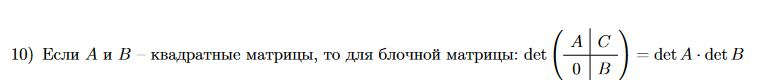
\includegraphics[width=\textwidth]{matrixProperty.JPG}

	\begin{flalign*}
		\forall A, \ B \
		\left(
		\left\{
		\begin{aligned}
			&A \in M_n \\
			&B \in M_n
		\end{aligned}
		\right.
		\longrightarrow
		det(A B) = det A \ det B
		\right)
	\end{flalign*}

	\begin{flalign*}
		det(A^{-1}) = det(A)^{-1}
	\end{flalign*}

	\begin{flalign*}
		\begin{array}{|rrrr|}
			1      & x_1    & \ldots & x_1^{n - 1} \\
			1      & x_2    & \ldots & x_2^{n - 1} \\
			\vdots & \vdots & \ddots & \vdots      \\
			1      & x_n    & \ldots & x_n^{n - 1}
		\end{array}
		-
		\text{определитель Вандермонда}.
	\end{flalign*}

	\begin{flalign*}
		\begin{array}{|rrrr|}
			1      & x_1    & \ldots & x_1^{n - 1} \\
			1      & x_2    & \ldots & x_2^{n - 1} \\
			\vdots & \vdots & \ddots & \vdots      \\
			1      & x_n    & \ldots & x_n^{n - 1}
		\end{array}
		=
		\prod_{1 \leq j < i \leq n}(x_i - x_j)
	\end{flalign*}

	\begin{flalign*}
		\forall A \
		\left(
		\exists B \
		B = A^{-1}
		\Leftrightarrow
		det A \neq 0
		\right)
	\end{flalign*}

	\section{Миноры, алгебраические дополнения и ранги}
	\begin{flalign*}
		\forall B, \ M, \ k \
		\left(
		\exists A \
		\left\{
		\begin{aligned}
			&A - \text{матрица из элементов матрицы} \ B \text{,} \\
			&\text{стоящих на пересечении} \ k \ \text{строк и} \ k \ \text{столбцов}. \\
			&M = det A
		\end{aligned}
		\right.
		\Leftrightarrow
		M - \text{минор} \ k \ \text{порядка матрицы} \ B.
		\right)
	\end{flalign*}

	\begin{flalign*}
		\forall B, \ M \
		\left(
		\exists A \
		\left\{
		\begin{aligned}
			&A - \text{матрица, на главной диагонали которой стоят} \\
			&\text{только все или не все элементы} \\
			&\text{главной диагонали} \ B. \\
			&M = det A
		\end{aligned}
		\right.
		\Leftrightarrow
		M - \text{главный минор матрицы} \ B.
		\right)
	\end{flalign*}

	\begin{flalign*}
		\forall A \
		Rg A - \text{ранг} \ A.
	\end{flalign*}

	\begin{flalign*}
		\forall A \
		Rg A = \text{наибольший порядок отличного от} \ 0 \ \text{минора матрицы} \ A.
	\end{flalign*}

	\begin{flalign*}
		\forall A \
		&Rg A
		= \\
		&\text{максимальное число линейно независимых строк}
		= \\
		&\text{максимальное число линейно независимых столбцов}.
	\end{flalign*}

	\begin{flalign*}
		\forall A, \ A' \
		\left(
		A' - \text{матрица, полученная из} \ A \ \text{элементарными преобразованиями}.
		\longrightarrow
		Rg A = Rg A'
		\right)
	\end{flalign*}

	\begin{flalign*}
		\forall A \
		\left(
		\exists n \
		\left\{
		\begin{aligned}
			&A \in M_n \\
			&Rg A = n
		\end{aligned}
		\right.
		\Leftrightarrow
		det A \neq 0
		\right)
	\end{flalign*}

	\begin{flalign*}
		\forall A \
		\left(
		\exists n \
		\left\{
		\begin{aligned}
			&A \in M_n \\
			&A_1, A_2, \ldots, A_n - \text{линейно независимые}.
		\end{aligned}
		\right.
		\Leftrightarrow
		det A \neq 0
		\right)
	\end{flalign*}

	\begin{flalign*}
		\forall A, \ M \
		\left(
		\left\{
		\begin{aligned}
			&M - \text{минор порядка} \ Rg A \ \text{матрицы} \ A. \\
			&M \neq 0
		\end{aligned}
		\right.
		\Leftrightarrow
		M - \text{базисный минор матрицы} \ A.
		\right)
	\end{flalign*}

	\begin{flalign*}
		\forall A, \ i \
		\left(
		A_i - \text{то, из чего составлен базисный минор матрицы} \ A.
		\longrightarrow
		A_i - \text{базисный}.
		\right)
	\end{flalign*}

	\begin{flalign*}
		\forall A, \ i \
		\left(
		\overline{A_i - \text{базисный}}.
		\longrightarrow
		A_i - \text{линейная комбинация базисных матрицы} \ A.
		\right)
	\end{flalign*}

	\begin{flalign*}
		\forall M, \ M' \
		\left(
		\exists A \
		\left\{
		\begin{aligned}
			&M - \text{минор матрицы} \ A. \\
			&M' - \text{минор, составленный} \\
			&\text{из тех же строк и столбцов, что и} \ M \text{,} \\
			&\text{и добавленных одной строки и одного столбца} \\
			&\text{матрицы} \ A.
		\end{aligned}
		\right.
		\Leftrightarrow
		M' - \text{окаймляющий минор} \ M.
		\right)
	\end{flalign*}

	\begin{flalign*}
		\forall A, \ M, \ k \
		\left(
		\left\{
		\begin{aligned}
			&M - \text{минор} \ k \ \text{порядка матрицы} \ A. \\
			&\text{Все окаймляющие миноры минора} \ M = 0
		\end{aligned}
		\right.
		\longrightarrow
		Rg A = k
		\right)
	\end{flalign*}

	\begin{flalign*}
		\forall A, \ B, \ M \
		\left(
		\left\{
		\begin{aligned}
			&A - \text{матрица из элементов матрицы} \ B \text{,} \\
			&\text{кроме строк и столбцов} \ B \text{,} \\
			&\text{из которых составлен минор} \ M. \\
			&M' = det A
		\end{aligned}
		\right.
		\Leftrightarrow
		M' - \text{дополнительный минор к минору} \ M.
		\right)
	\end{flalign*}

	\begin{flalign*}
		\forall M, \ M^* \
		\left(
		\exists A, \ \alpha, \ n \
		\left\{
		\begin{aligned}
			&A = A_{n} \\
			&\alpha = \text{сумма номеров строк и столбцов} \ A \text{,} \\
			&\text{из которых составлен минор} \ M. \\
			&M' - \text{дополнительный минор к минору} \ M. \\
			&M^* = (-1)^\alpha M'
		\end{aligned}
		\right.
		\Leftrightarrow
		\begin{aligned}
			&M^* - \text{алгебраическое дополнение} \\
			&\text{к минору} \ M.
		\end{aligned}
		\right)
	\end{flalign*}

	\begin{flalign*}
		\forall A, \ i, \ j \
		M_{i j} - \text{минор элемента} \ [A]_{i j} \ \text{матрицы} \ A.
	\end{flalign*}

	\begin{flalign*}
		\forall A, \ n, \ i, \ j \
		\left(
		\left\{
		\begin{aligned}
			&A = A_{n} \\
			&A - \text{матрица из элементов матрицы} \ B \text{,} \\
			&\text{кроме строки} \ i \ \text{и столбца} \ j.
		\end{aligned}
		\right.
		\Leftrightarrow
		det A = M_{i j}
		\right)
	\end{flalign*}

	\begin{flalign*}
		\forall A, \ i, \ j \
		A_{i j} - \text{алгебраическое дополнение элемента} \ [A]_{i j}.
	\end{flalign*}

	\begin{flalign*}
		\forall A,\ i, \ j \
		A_{i j} = (-1)^{i + j} M_{i j}
	\end{flalign*}

	\section{Форматы матриц}
	\textbf{Ведущий элемент} - это
	первый ненулевой элемент строки.

	\textbf{Ступенчатый вид матрицы} - это
	матрица, номера столбцов ведущих элементов которой
	возрастают, а нулевые строки, если они есть,
	расположены внизу.

	\textbf{Улучшенный (приведённый, канонический) ступенчатый вид матрицы} - это
	ступенчатый вид матрицы, в котором все ведущие
	элементы - единицы, над которыми в столбце все
	элементы - нули.

	Любую матрицу элементарными преобразованиями
	можно привести к улучшенному ступенчатому виду.

	\begin{flalign*}
		\forall A, \ B, \ C \
		\left(
		\exists m, \ r, \ n \
		\left\{
		\begin{aligned}
			&B \in M_{m \times r} \\
			&C \in M_{r \times n} \\
			&r = Rg B = Rg C \\
			&A = B C
		\end{aligned}
		\right.
		\Leftrightarrow
		B C - \text{скелетное разложение} \ A.
		\right)
	\end{flalign*}

	\begin{flalign*}
		\forall A, \ B, \ C \
		\left(
		\exists m, \ r, \ n \
		\left\{
		\begin{aligned}
			&B - \text{нижняя треугольная матрица матрицы}. \\
			&C - \text{верхняя треугольная матрица матрицы}. \\
			&A = B C
		\end{aligned}
		\right.
		\Leftrightarrow
		B C - \text{LU разложение} \ A.
		\right)
	\end{flalign*}

	\begin{flalign*}
		\forall A \
		\left(
		A - \text{строго регулярная}.
		\Leftrightarrow
		A - \text{имеет LU разложение}.
		\right)
	\end{flalign*}

	\section{СЛАУ относительно матриц}
	\begin{flalign*}
		\forall a \
		\left(
		\left\{
		\begin{aligned}
			&a - \text{СЛАУ}. \\
			&a - \text{имеет решение}.
		\end{aligned}
		\right.
		\longrightarrow
		a - \text{совместная}.
		\right)
	\end{flalign*}

	\begin{flalign*}
		\forall a \
		\left(
		\left\{
		\begin{aligned}
			&a - \text{СЛАУ}. \\
			&a - \text{не имеет решений}.
		\end{aligned}
		\right.
		\longrightarrow
		a - \text{несовместная}.
		\right)
	\end{flalign*}

	\begin{flalign*}
		\forall A, \ x, \ b \
		\left(
		Ax = b - \text{СЛАУ}.
		\longrightarrow
		\forall i \
		\left\{
		\begin{aligned}
			&\Delta_i = det(A_1, A_2, \ldots, A_{i - 1}, B, A{i + 1}, \ldots, A_n) \\
			&\Delta = det A \\
			&x_i = \frac{\Delta_i}{\Delta}
		\end{aligned}
		\right.
		\right)
	\end{flalign*}

	\begin{flalign*}
		\forall A, \ x, \ b \
		\left(
		\exists i \
		\left\{
		\begin{aligned}
			&Ax = b - \text{СЛАУ}. \\
			&\Delta = 0 \\
			&\Delta_{i} \neq 0
		\end{aligned}
		\right.
		\longrightarrow
		Ax = b - \text{несовместная}.
		\right)
	\end{flalign*}

	\begin{flalign*}
		\forall A, \ x, \ b \
		\left(
		\left\{
		\begin{aligned}
			&Ax = b - \text{СЛАУ}. \\
			&\Delta \neq 0
		\end{aligned}
		\right.
		\longrightarrow
		\left\{
		\begin{aligned}
			&Ax = b - \text{совместная}. \\
			&Ax = b - \text{имеет единственное решение}.
		\end{aligned}
		\right.
		\right)
	\end{flalign*}

	\textbf{Теорема Кронекера-Капелли:}
	\begin{flalign*}
		\forall A, \ b \
		\left(
		Rg A = Rg(A | b)
		\Leftrightarrow
		\exists x \
		Ax = b - \text{совместная}.
		\right)
	\end{flalign*}

	\begin{flalign*}
		\forall A, \ l, \ n \
		\left(
		\left\{
		\begin{aligned}
			&A_l, A_{l + 1}, \ldots, A_{l + n - RgA - 1} - \text{л.н.з. столбцы}. \\
			&A_l, A_{l + 1}, \ldots, A_{l + n - RgA - 1} - \text{решения} \ Ax = 0. \\
			&n - \text{число неизвестных}.
		\end{aligned}
		\right.
		\Leftrightarrow
		\begin{aligned}
			&A_l, A_{l + 1}, \ldots, A_{l + n - RgA - 1} - \\
			&\text{фундаментальная система} \\
			&\text{решений (ФСР)} \ Ax = 0.
		\end{aligned}
		\right)
	\end{flalign*}

	\begin{flalign*}
		\forall A, \ x \
		\left(
		Ax = 0
		\longrightarrow
		\exists C \
		C - \text{ФСР} \ Ax = 0.
		\right)
	\end{flalign*}

	\begin{flalign*}
		\forall C, \ x \
		\exists n \
		\left(
		\exists m \
		C_{m \times n} - \text{ФСР} \ Ax = 0.
		\longrightarrow
		x = \alpha_1 C_1 + \ldots + \alpha_n C_n.
		\right)
	\end{flalign*}

	\begin{flalign*}
		\forall C, \ x \
		\exists \sequence{\alpha_n}, \ n \
		\left(
		\exists m \
		\left\{
		\begin{aligned}
			&C_{m \times n} - \text{ФСР} \ Ax = 0. \\
			&Ax' = b
		\end{aligned}
		\right.
		\longrightarrow
		x' + \alpha_1 C_1 + \ldots + \alpha_n C_n - \text{все решения} \ Ax = b.
		\right)
	\end{flalign*}

	\chapter{Векторы}
	\begin{flalign*}
		\forall \overrightarrow{a}, \  \overrightarrow{b} \
		\left(
		\overrightarrow{a}, \overrightarrow{b} - \text{лежат на одной прямой или на параллельных}.
		\Leftrightarrow
		\overrightarrow{a}, \overrightarrow{b} - \text{коллинеарны}.
		\right)
	\end{flalign*}

	\begin{flalign*}
		\forall \overrightarrow{a}, \  \overrightarrow{b}, \ \overrightarrow{c} \
		\left(
		\begin{aligned}
			&\overrightarrow{a}, \overrightarrow{b}, \overrightarrow{c} - \text{лежат на прямых,} \\
			&\text{параллельных некоторой плоскости}.
		\end{aligned}
		\Leftrightarrow
		\overrightarrow{a}, \overrightarrow{b}, \overrightarrow{c} - \text{компланарны}.
		\right)
	\end{flalign*}

	\begin{flalign*}
		\forall \overrightarrow{a}, \  \overrightarrow{b} \
		\left(
		\left\{
		\begin{aligned}
			&\overrightarrow{a} \upuparrows \overrightarrow{b} \\
			&\left\lvert \overrightarrow{a} \right\rvert = \left\lvert \overrightarrow{b} \right\rvert
		\end{aligned}
		\right.
		\Leftrightarrow
		\overrightarrow{a} = \overrightarrow{b}
		\right)
	\end{flalign*}

	\begin{flalign*}
		\forall \overrightarrow{a}, \  \overrightarrow{b} \
		\left(
		\left\{
		\begin{aligned}
			&\overrightarrow{a} = \overrightarrow{b} \\
			&\text{Начало} \ \overrightarrow{a}, \ \text{начало} \ \overrightarrow{b} \ \text{лежат на одной прямой}.
		\end{aligned}
		\right.
		\Leftrightarrow
		\overrightarrow{a}, \overrightarrow{b} - \text{скользящие}.
		\right)
	\end{flalign*}

	\begin{flalign*}
		\forall \overrightarrow{a}, \  \overrightarrow{b} \
		\left(
		\left\{
		\begin{aligned}
			&\overrightarrow{a} = \overrightarrow{b} \\
			&\text{Начало} \ \overrightarrow{a} = \text{начало} \ \overrightarrow{b}
		\end{aligned}
		\right.
		\Leftrightarrow
		\overrightarrow{a}, \overrightarrow{b} - \text{связанные}.
		\right)
	\end{flalign*}

	\begin{flalign*}
		+ - \text{операция на векторах, обладающая коммутативным свойством.}
	\end{flalign*}

	\begin{flalign*}
		+ - \text{операция на векторах, обладающая ассоциативным свойством.}
	\end{flalign*}

	\begin{flalign*}
		* - \text{операция на векторе и числе, обладающая коммутативным свойством.}
	\end{flalign*}

	\begin{flalign*}
		* - \text{операция на векторе и числе, обладающая ассоциативным свойством.}
	\end{flalign*}

	\begin{flalign*}
		&* - \text{операция на векторе и числе, обладающая дистрибутивным свойством c} \ + \\
		&\text{относительно векторов и относительно чисел.}
	\end{flalign*}

	\begin{flalign*}
		\forall \overrightarrow{b} \
		\left(
		\overrightarrow{b} \neq 0
		\Leftrightarrow
		\exists \overrightarrow{a} \
		\left\lvert a \right\rvert * \cos \angle \left(\overrightarrow{a}, \overrightarrow{b}\right) - \text{ортогональная проекция} \ \overrightarrow{a} \ \text{на направление} \ \overrightarrow{b}.
		\right)
	\end{flalign*}

	\begin{flalign*}
		\text{Ортогональная проекция уважает сложение векторов.}
	\end{flalign*}

	\begin{flalign*}
		\text{Ортогональная проекция уважает умножение вектора на число.}
	\end{flalign*}

	\begin{flalign*}
		\forall \overrightarrow{a}, \ \overrightarrow{b} \
		\left(\overrightarrow{a}, \overrightarrow{b}\right)
		=
		\left\lvert \overrightarrow{a} \right\rvert \left\lvert \overrightarrow{b} \right\rvert \cos \varphi
	\end{flalign*}

	\begin{flalign*}
		\forall \overrightarrow{a}, \ \overrightarrow{b} \
		\left(\overrightarrow{a}, \overrightarrow{b}\right)
		=
		\left(\overrightarrow{b}, \overrightarrow{a}\right)
	\end{flalign*}

	\begin{flalign*}
		\forall \overrightarrow{a}, \ \overrightarrow{b} \
		\left(\alpha \overrightarrow{a}, \overrightarrow{b}\right)
		=
		\alpha \left(\overrightarrow{a}, \overrightarrow{b}\right)
	\end{flalign*}

	\begin{flalign*}
		\forall \overrightarrow{a}, \ \overrightarrow{b} \
		\left(\overrightarrow{a} + \overrightarrow{b}, \overrightarrow{c}\right)
		=
		\left(\overrightarrow{a}, \overrightarrow{c}\right) + \left(\overrightarrow{b}, \overrightarrow{c}\right)
	\end{flalign*}

	\begin{flalign*}
		\forall \overrightarrow{a}\
		\left(
		\overrightarrow{a} \neq 0
		\Leftrightarrow
		0 < \left(\overrightarrow{a}, \overrightarrow{a}\right)
		\right)
	\end{flalign*}

	\begin{flalign*}
		\forall \overrightarrow{a}\
		\left(
		\overrightarrow{a} = 0
		\Leftrightarrow
		0 = \left(\overrightarrow{a}, \overrightarrow{a}\right)
		\right)
	\end{flalign*}

	\begin{flalign*}
		\forall \overrightarrow{a_1}, \ \overrightarrow{a_2}, \ \ldots, \ \overrightarrow{a_k} \
		\left(
		\forall \overrightarrow{b} \
		\left\{
		\begin{aligned}
			&\overrightarrow{a_1}, \overrightarrow{a_2}, \ldots, \overrightarrow{a_k} - \text{л.н.з.} \\
			&\overrightarrow{b} - \text{линейная комбинация} \ \overrightarrow{a_1}, \overrightarrow{a_2}, \ldots, \overrightarrow{a_k}.
		\end{aligned}
		\right.
		\Leftrightarrow
		\overrightarrow{a_1}, \overrightarrow{a_2}, \ldots, \overrightarrow{a_k} - \text{базис}.
		\right)
	\end{flalign*}

	\begin{flalign*}
		\forall \overrightarrow{a_1}, \ \overrightarrow{a_2}, \ \ldots, \ \overrightarrow{a_k} \
		\left(
		\forall \overrightarrow{b} \
		\left\{
		\begin{aligned}
			&\overrightarrow{a_1}, \overrightarrow{a_2}, \ldots, \overrightarrow{a_k} - \text{базис} \\
			&i = j \longrightarrow (a_i, a_j) = 1 \\
			&i \neq j \longrightarrow (a_i, a_j) = 0
		\end{aligned}
		\right.
		\Leftrightarrow
		\overrightarrow{a_1}, \overrightarrow{a_2}, \ldots, \overrightarrow{a_k} - \text{ортонормированный базис (ОНБ)}.
		\right)
	\end{flalign*}

	\begin{flalign*}
		\forall \overrightarrow{a}, \ \overrightarrow{b} \
		\left(\overrightarrow{a}, \overrightarrow{b}\right) = a_x b_x + a_y b_y + \ldots \ \text{в ОНБ}.
	\end{flalign*}

	\begin{flalign*}
		\text{Г} - \text{матрица Грама}.
	\end{flalign*}

	\begin{flalign*}
		\forall \overrightarrow{e_1}, \ \overrightarrow{e_2}, \ \overrightarrow{e_3} \
		\left(
		\overrightarrow{e_1}, \overrightarrow{e_2}, \overrightarrow{e_3} - \text{базис}.
		\Leftrightarrow
		\left(
		\begin{array}{rrr}
			\left(\overrightarrow{e_1}, \overrightarrow{e_1}\right) & \left(\overrightarrow{e_1}, \overrightarrow{e_2}\right) & \left(\overrightarrow{e_1}, \overrightarrow{e_3}\right) \\
			\left(\overrightarrow{e_2}, \overrightarrow{e_2}\right) & \left(\overrightarrow{e_2}, \overrightarrow{e_2}\right) & \left(\overrightarrow{e_2}, \overrightarrow{e_3}\right) \\
			\left(\overrightarrow{e_3}, \overrightarrow{e_1}\right) & \left(\overrightarrow{e_3}, \overrightarrow{e_2}\right) & \left(\overrightarrow{e_3}, \overrightarrow{e_3}\right)
		\end{array}
		\right)
		=
		\text{Г}
		\right)
	\end{flalign*}

	\begin{flalign*}
		\forall \ldots
		\left(
		\left\{
		\begin{aligned}
			&\overrightarrow{e_1}, \overrightarrow{e_2}, \overrightarrow{e_3} - \text{базис}. \\
			&\overrightarrow{a} = a_1 \overrightarrow{e_1} + a_2 \overrightarrow{e_2} + a_3 \overrightarrow{e_3} \\
			&\overrightarrow{b} = b_1 \overrightarrow{e_1} + b_2 \overrightarrow{e_2} + b_3 \overrightarrow{e_3}
		\end{aligned}
		\right.
		\longrightarrow
		\left(\overrightarrow{a}, \overrightarrow{b}\right)
		=
		\left(
		\begin{array}{rrr}
			a_1 & a_2 & a_3
		\end{array}
		\right)
		\text{Г}
		\left(
		\begin{array}{r}
			b_1 \\
			b_2 \\
			b_3
		\end{array}
		\right)
		\right)
	\end{flalign*}

	\begin{flalign*}
		\forall \overrightarrow{i}, \ \overrightarrow{j}, \ \overrightarrow{k} \
		\left(
		\overrightarrow{i}, \overrightarrow{j}, \overrightarrow{k} - \text{ортогональный базис}.
		\Leftrightarrow
		\forall \overrightarrow{a} \
		\begin{aligned}
			&cos \angle \left(\overrightarrow{a}, \overrightarrow{i}\right), cos \angle \left(\overrightarrow{a}, \overrightarrow{j}\right), cos \angle \left(\overrightarrow{a}, \overrightarrow{j}\right) - \\
			&\text{направляющие косинусы} \ \overline{a}.
		\end{aligned}
		\right)
	\end{flalign*}

	\begin{flalign*}
		\forall \overrightarrow{i}, \ \overrightarrow{j}, \ \overrightarrow{k} \
		\left(
		\overrightarrow{i}, \overrightarrow{j}, \overrightarrow{k} - \text{ортогональный базис}.
		\Leftrightarrow
		\forall \overrightarrow{a} \
		cos^2 \angle \left(\overrightarrow{a}, \overrightarrow{i}\right) + cos^2 \angle \left(\overrightarrow{a}, \overrightarrow{j}\right) + cos^2 \angle \left(\overrightarrow{a}, \overrightarrow{k}\right) = 1
		\right)
	\end{flalign*}

	\begin{flalign*}
		\forall \overrightarrow{a}, \ \overrightarrow{b}, \ \overrightarrow{c}
		\left(
		\text{Со стороны} \ \overrightarrow{c} \ \text{кратчайший поворот от} \ \overrightarrow{a} \ \text{к} \ \overrightarrow{b} \text{против часовой}.
		\Leftrightarrow
		\overrightarrow{a}, \overrightarrow{b}, \overrightarrow{c} - \text{правая}.
		\right)
	\end{flalign*}

	\begin{flalign*}
		\left\lvert \overrightarrow{a} \times \overrightarrow{b} \right\rvert = \left\lvert \overrightarrow{a} \right\rvert \left\lvert \overrightarrow{b} \right\rvert \sin \angle \left(\overrightarrow{a}, \overrightarrow{b}\right)
	\end{flalign*}

	\begin{flalign*}
		\forall \overrightarrow{a}, \ \overrightarrow{b}, \ \overrightarrow{c} \
		\left(
		\overrightarrow{c} = \overrightarrow{a} \times \overrightarrow{b}
		\Leftrightarrow
		\overrightarrow{a}, \overrightarrow{b}, \overrightarrow{c} - \text{правая}.
		\right)
	\end{flalign*}

	\begin{flalign*}
		\forall \overrightarrow{a}, \ \overrightarrow{b} \
		\left(
		\overrightarrow{a} \times \overrightarrow{b} = 0
		\Leftrightarrow
		\overrightarrow{a} \Vert \overrightarrow{b}
		\right)
	\end{flalign*}

	\begin{flalign*}
		\forall \overrightarrow{a}, \ \overrightarrow{b} \
		\overrightarrow{a} \times \overrightarrow{b} \bot \overrightarrow{a}
	\end{flalign*}

	\begin{flalign*}
		\forall \overrightarrow{a}, \ \overrightarrow{b} \
		\overrightarrow{a} \times \overrightarrow{b} = -\overrightarrow{b} \times \overrightarrow{a}
	\end{flalign*}

	\begin{flalign*}
		\left(\alpha \overrightarrow{a}\right) \times \overrightarrow{b} = \alpha \left(\overrightarrow{a} \times \overleftrightarrow{b} \right)
	\end{flalign*}

	\begin{flalign*}
		&\times - \text{операция на векторах, обладающая дистрибутивным свойством c} \ + \\
		&\text{относительно векторов.}
	\end{flalign*}

	\begin{flalign*}
		\forall \overrightarrow{a}, \ \overrightarrow{b}, \ \overrightarrow{c} \
		\left(
		0 < \left(\overrightarrow{a} \times \overrightarrow{b}, \overrightarrow{c}\right)
		\longrightarrow
		\overrightarrow{a}, \overrightarrow{b}, \overrightarrow{c} - \text{правая}.
		\right)
	\end{flalign*}

	\begin{flalign*}
		\forall \overrightarrow{a}, \ \overrightarrow{b}, \ \overrightarrow{c} \
		\left(
		\left(\overrightarrow{a} \times \overrightarrow{b}, \overrightarrow{c}\right) < 0
		\longrightarrow
		\overrightarrow{a}, \overrightarrow{b}, \overrightarrow{c} - \text{левая}.
		\right)
	\end{flalign*}

	\begin{flalign*}
		\forall \overrightarrow{a}, \ \overrightarrow{b}, \ \overrightarrow{c} \
		\left(
		\left(\overrightarrow{a} \times \overrightarrow{b}, \overrightarrow{c}\right) = 0
		\Leftrightarrow
		\overrightarrow{a}, \overrightarrow{b}, \overrightarrow{c} - \text{компланарны}.
		\right)
	\end{flalign*}

	\begin{flalign*}
		\forall \overrightarrow{a}, \ \overrightarrow{b}, \ \overrightarrow{c} \
		\left(\overrightarrow{a} \times \overrightarrow{b}, \overrightarrow{c}\right)
		=
		\begin{array}{|rrr|}
			a_x & a_y & a_z \\
			b_x & b_y & b_z \\
			c_x & c_y & c_z
		\end{array} \
		\text{в ОНБ}.
	\end{flalign*}

	\begin{flalign*}
		\forall \overrightarrow{i}, \ \overrightarrow{j}, \ \overrightarrow{k} \
		\left(
		\exists a, \ b, \ c \
		\left\{
		\begin{aligned}
			&\overrightarrow{i}, \overrightarrow{j}, \overrightarrow{k} - \text{ОНБ}. \\
			&O
			=
			\left(
			\begin{array}{r}
				a \\
				b \\
				c
			\end{array}
			\right)
		\end{aligned}
		\right.
		\Leftrightarrow
		\begin{aligned}
			&(O \times \overrightarrow{i}, \overrightarrow{j}, \overrightarrow{k}) - \text{прямоугольная} \\
			&\text{декартова система координат (ПДСК)}.
		\end{aligned}
		\right)
	\end{flalign*}
\end{document}
